\documentclass[10pt,a4paper]{article}
\usepackage{fontspec,amsmath,amssymb,amsthm,mathtools,graphicx,bm}
\usepackage[margin=22mm]{geometry}
\usepackage[bookmarks=false]{hyperref}
\setlength{\emergencystretch}{3em}
\title{Exponential size lower bounds for k-DNF Resolution from boundary expansion}
\author{Anastasia Sofronova, Dmitry Sokolov}
\date{doi:10.4230/LIPIcs.CCC.2025.32; CC BY 4.0}
\begin{document}
\maketitle
\noindent\textit{Editorial note.} Editable TeX faithfully converted from official CC BY HTML prose/math alttext. The official HTML/PDF originals are included. Only general Theorem 3 counts; the linear-system reformulation and random-CNF applications are retained without separate counts. The explicit expansion constants and asymptotic parameter condition remain as printed by the authors.\par\medskip
\noindent\textit{Editorial note.} SVG assembly correction: official HTML object graphics restored at their original paragraph positions. Original SVGs, faithful vector PDF conversions and URL/license ledger are included; all existing author text and captions are retained.\par\medskip
\noindent\textit{Allowed standard prerequisites (editorial).}\begin{itemize}
\item Standard resolution, CNF dependency graphs and probability bounds. All author-local definitions and proof support retained.
\end{itemize}\medskip


\par\medskip\noindent\textbf{
1 Introduction}\par




Proof complexity studies whether there are efficient certificates for the unsatisfiability of boolean
formulas. While satisfiability is easy to certify (one could consider a satisfying assignment if it
exists), the question whether there exist polynomial-size proofs of unsatisfiability for every
boolean formula remains a huge open problem in complexity theory. The non-existence of such proofs in any
proof system would separate the classes ${\mathsf{NP}}$ and ${\mathsf{coNP}}$. According to Cook’s program, the idea is to prove
lower bounds for stronger and stronger proof systems, so eventually we would be able to do it in a general
case.\par




One of the difficulties with implementing this plan is the shortage of candidates for hard families of
formulas. The intuition here is that any unsatisfiable example a person could invent is most likely
accompanied with some natural reasons for its unsatisfiability (e.g. it is not hard to argue in natural
language that Pigeonhole Principle or Tseitin formulas are unsatisfiable). One can formalize these
reasons to try and produce an efficient proof in some proof system. The same intuition suggests to look
at distributions of formulas for the hard candidates. As of now, there are three known distribution-based
options:\par


\begin{itemize}


\item[] 
$\blacksquare$ 


random $\Delta$-CNFs;\par





\item[] 
$\blacksquare$ 


pseudorandom generators (aka proof complexity generators);\par





\item[] 
$\blacksquare$ 


clique formulas.\par





\end{itemize}




In this work, we focus on the first one. Random $\Delta$-CNF formulas are an important and popular
object in various areas of the complexity
theory. These formulas are generated as a random subset of $m$ clauses over $n$ variables.\par



% SOURCE-ID Thmtheorem1


\par\medskip\noindent\textbf{
\textbf{Definition 1}\textbf{.}
}\par



\emph{Let $\varphi(m,n,\Delta)$ denote the distribution of random $\Delta$-CNF on $n$ variables
obtained by sampling $m$ clauses of width $\Delta$ (out of the $\binom{n}{\Delta}2^{\Delta}$
possible clauses) uniformly at random with replacement.}\par




\emph{We denote a \textbf{clause density} by $\chi\coloneqq\frac{m}{n}$.}\par



% END-SOURCE-ID Thmtheorem1



It is a well-known fact that such formulas are unsatisfiable with high probability (whp), if $m$ is large
enough.\par



% SOURCE-ID Thmtheorem2


\par\medskip\noindent\textbf{
\textbf{Lemma 2}\textbf{ }(Chvátal–Szemerédi, [15])\textbf{.}
}\par



\emph{For any $\Delta\geq 3$ whp $\varphi\sim\varphi(m,n,\Delta)$ is unsatisfiable if $m\geq\ln 2\cdot 2^{\Delta}n$.}\par



% END-SOURCE-ID Thmtheorem2



In other words, for each $\Delta$ there is a density threshold $c_{\Delta}$ such that if $\chi>c_{\Delta}$ then whp the formula is unsatisfiable and if $\chi<c_{\Delta}$ then whp the formula is
satisfiable.\par




\par\medskip\noindent\textbf{The mystery of density.}\par




A common belief is that solving the satisfiability problem for random $\Delta$-CNF formulas
near the density threshold is hard. At the same time if we sample too many clauses, say
$m\gg n^{\Delta-1}$, then whp our formula will contain \emph{a local contradiction}, i.e. there will
be a subformula on small number of variables that is unsatisfiable and even tree-like Resolution
may efficiently certify it. Even for SAT solvers clause density helps to reduce the running time, in
particular, the running time of ordered $\mathrm{DLL}$ procedure is upper bounded by
$\exp\left(\mathcal{O}\left(\frac{n}{\chi^{1/(\Delta-2)}}\right)\right)$ [11]. And yet there is
a certain gap between the satisfiability threshold and the density increase that is noticeable by the
proof systems in the sense that it reduces the size of the proof. An exciting recent line of work
[6, 32, 1, 23] provides strong refutation algorithms for
random and semi-random CNFs for certain
high-density regimes. Such algorithms found their applications in combinatorics and coding theory
[7, 26]. Exploring different density regimes in various proof system thus seems
crucial.\par




Feige’s conjecture [18] states: no polynomial time algorithm may \emph{prove} whp the
unsatisfiability of a random $\mathcal{O}\left(1\right)$-CNF formula with arbitrary large constant clause density. This
assumption of hardness on average implies the inapproximability of many NP-hard problems, such as vertex
covering, DNF PAC learning, etc.\par




The sequence of papers that starts with the classical lower bounds by Chvátal and Szemerédi
[15] shows the hardness of random $\Delta$-CNF formulas in Resolution for various regimes of
density. In [15] the authors show that for any fixed $\chi\geq 2^{\Delta}\ln 2$ there is a
constant $\kappa(\chi)$ such that random $k$-SAT requires length $\exp(\kappa(\chi)n)$ with high
probabilty. But $\kappa$ decays doubly-exponentially as $\chi$ increases and lower bound becomes trivial
when $m\gg n\log^{1/4}n$. Later lower bounds by Ben-Sasson–Wigderson [14] and by Beame et al
[11] reduced the decay in $\kappa$ to polynomial in $\chi$. Later Ben-Sasson [12]
improved the polynomial in the dependency on $\chi$. Similar type of dependencies on the density is known
also for several other proof systems: Polynomial Calculus [13, 5], Sum-of-Squares
[22]. $\mathrm{Res}(k)$ proof system is a notable exception, and we have lower bounds only for
density near the satisfiability threshold.\par




From the proof complexity point of view, random $\Delta$-CNFs are one of the most promising candidates to
be hard for any proof system. We know many lower bounds for random formulas even in powerful proof
systems like Sum-of-Squares. Such lower bounds are out of reach for other candidates like PRG formulas
[4, 33] or Clique formulas [8, 31, 17]. We mention known results
for random formulas in Section 1.1.\par





\par\medskip\noindent\textbf{
1.1 Prior Results}\par




The following table summarizes known facts about the complexity of random $\Delta$-CNFs in different
proof systems.

\par






\textbf{Proof system}




\textbf{Polynomial upper bound}




\textbf{Lower bound} $2^{n^{\varepsilon}}$








Resolution




$m>\frac{n^{\Delta-1}}{\log^{\Delta-2}n}$ [11]




$m<n^{\frac{\Delta}{2}-o(1)}$ [12]






Polynomial Calculus





$m=\mathcal{O}\left(n\right),\Delta\geq 3$ [13]
$m={\mathsf{poly}}(n),\Delta=3$ [5]






Sum-of-Squares




$\Delta=k,m=\widetilde{\mathcal{O}}(n^{\frac{k}{2}})$,
[6, 32, 1, 23]




$m={\mathsf{poly}}(n),\Delta=\mathcal{O}\left(1\right)$ [22], [34], [27]






Cutting Planes





$m={\mathsf{poly}}(n),\Delta=\Omega(\log n)$
[25], [20], [37]






${\mathsf{TC}}_{0}$-Frege




$\Delta=3$, $m>n^{1.4}$ [19], [29]




$\times$






$\mathrm{Res}(k)$





$m=\mathcal{O}\left(n\right),\Delta\geq 3,k=2$ [9]
$m=\mathcal{O}\left(n\right),\Delta\geq 3,k=\mathcal{O}\left(\sqrt{\frac{\log n%
}{\log\log n}}\right)$
[3]
$m=n^{7/6},\Delta=\mathcal{O}\left(k^{2}\right),k=\mathcal{O}\left(1\right)$ [35]








To clarify the comparison of these results, let us note here than Resolution is a strictly weaker system
than all the others present in the table. ${\mathsf{TC}}_{0}$ models every other system present in the table, expect
Sum-of-Squares, for which their relationship is not known. Everything else is not comparable (depending
on the specific field for algebraic systems).\par




The big long-standing open problem in proof complexity is to show ${\mathsf{AC}}_{0}$-Frege lower bounds for random
$\Delta$-CNF formulas. Even for non-constant $\Delta$ and depth-$2$ Frege this problem seems to be out of
reach for current techniques. The current frontier in this direction is $\mathrm{Res}(k)$ proof system that was
introduced by Krajíček [28]. This is a subsystem of depth-$2$ Frege that uses
$k$-DNF formulas as proof lines (see Section 2) rather than general DNF formulas that are
used by depth-$2$ Frege. In fact, it would be enough to have a \emph{robust} (i.e. stable under
restrictions of formulas) lower bound for $k=\log^{1+\varepsilon}n$ to extend it to all $k$’s and,
therefore, to depth-$2$ Frege using random restriction, so the gap between current state-of-the-art and
this threshold might very well be breachable. Here by robust we mean a technique that is not tailored
precisely to a specific unsatisfiable family, but that allows a certain degree of freedom in choosing a
hard formula.\par




\par\medskip\noindent\textbf{Known techniques.}\par




All known techniques for proving lower bounds on the proof systems that
are at least as powerful as $\mathrm{Res}(2)$ are based on the restriction argument. In other words we choose a
random partial assignment to the variables from a carefully chosen distribution, hit the formula and the
proof by this assignment in order to get an extremely structured proof and leave the restricted formula
hard for such proofs. In particular, ${\mathsf{AC}}_{0}$-Frege \emph{transforms} into a resolution proof under large
partial assignments (we should assign $n-o(n)$ number of variables); this method is also known as
switching lemma [2, 10, 24]. We do not know how to make such an assignment and keep
random $\Delta$-CNF formula hard for resolution. All known hardness results for refuting random formulas
in $\mathrm{Res}(k)$ are trying to avoid this problem in different ways and require different properties of
random formulas. The key tool is the Small Restriction Switching Lemma, which assigns $\varepsilon n$
number of variables and reduces a $\mathrm{Res}(k)$ proof to a Resolution proof.\par


\begin{itemize}


\item[] 
$\blacksquare$ 


In [35] the authors use the fact that for $\Delta\gtrsim k^{2}$ it is
possible to use the uniform distribution on a certain set of partial restrictions and keep
the restricted formula hard for Resolution. This result holds
in case of clause density at most $\chi=n^{1/6}$ and $k$ an absolute constant. This lower
bound is not \emph{uniform} in terms of choice of the proof system. In other words, if we want to
state that “there is a distribution on formulas that is hard for $\mathrm{Res}(k)$ proof systems for all
constant $k$”, we would need to purge the dependence between $\Delta$ and $k$.\par





\item[] 
$\blacksquare$ 


Alekhnovich in [3] shows the solution for this problem. The distribution over
partial assignments makes use of the structure of the dependency graph of the formula, but for the
analysis it was required that this graph has low right degree of all vertices (in other words, any
variable should appear in constant number of clauses). This requirement may be achieved only in
case of constant clause density of a random formula. $k$ in this setup is allowed to be at most
$\mathcal{O}\left(\sqrt{\frac{\log n}{\log\log n}}\right)$.\par





\end{itemize}


Both papers in addition require the dependency graph be an expander, which is a standard property for the
analysis of hardness (that is almost “necessary”, since we have to argue that there are no local
unsatisfiable subformulas).\par




Another relevant work is Razborov’s improved small-set switching lemma [33]. Though it builds
on an improved technique from [35], the formulas considered
(pseudorandom generators) are quite different, so it is not clear if this result is directly comparable
with ours.\par






\par\medskip\noindent\textbf{
1.2 Our Results}\par




We suggest a new technique that helps us to extend and unify both mentioned lower bounds. Our results
use only the fact that the dependency graph of a formula is a good enough expander. More formally, we
show the following in Section 5.\par




% SOURCE-ID Thmtheorem3


\par\medskip\noindent\textbf{
\textbf{Theorem 3}\textbf{.}
}\par



\emph{Let $\varphi$ be a $\Delta$-CNF formula such that its dependency graph $G$ is an $(r,\Delta,0.95\Delta)$-boundary expander. Then for any $\delta>0$ if:}\par


\[\begin{gathered}
n^{\delta}\left(\frac{n}{0.4r}\right)^{20k^{2}}=o(r/k)
\end{gathered}\]


\emph{then any $\mathrm{Res}(k)$ proof of $\varphi$ has size at least $2^{n^{\delta}}$.}\par



% END-SOURCE-ID Thmtheorem3




In Section 6 we show the following corollaries:\par


\begin{itemize}


\item[] 
$\blacksquare$ 


an exponential lower bound for any constant $k$, $\Delta=\mathcal{O}\left(1\right)$ in case $m={\mathsf{poly}}(n)$
(improvement of the result of Segerlind, Buss, Impagliazzo [35]);\par





\item[] 
$\blacksquare$ 


an exponential lower bound for $k=\mathcal{O}\left(\sqrt{\log n}\right)$, $\Delta=\mathcal{O}\left(1\right)$ in case $m=\mathcal{O}\left(n\right)$ (improvement of the result of Alekhnovich [3]).\par





\end{itemize}




We would like to emphasize that this result is the first that provides a lower bound on the $\mathrm{Res}(k)$
proofs for the constant $\Delta$ independent on $k$ and polynomially large clause density $m={\mathsf{poly}}(n)$.\par




As a weakness of our results, we should mention the fact that the constant $\Delta$ should be big enough
for the dependency graph of the formula to be an expander with good parameters. Naive computations say
that $\Delta\approx 100$ is enough (see Section C). We did not try to optimize
this constant, since we do not see the way to achieve the best possible value $3$ (like in
[3]).\par




We describe our technique below.\par




\par\medskip\noindent\textbf{Our technique.}\par




We follow the ideas of random restriction technique
[35, 3].\par




\begin{enumerate}


\item[] 
1. 


Given a $\Delta$-CNF formula $\varphi$ on $n$ variables and $m$ clauses, we assume that
a dependency graph (clauses–variables) is a good enough expander (this holds with probability $1-o(1)$ for random formulas).\par





\item[] 
2. 


For the sake of contradiction assume that there is a small $\mathrm{Res}(k)$-proof $\pi$ of $\varphi$. We
would like to create a partial assignment $\rho$ such that:\par


\begin{itemize}


\item[] 
$\blacksquare$ 


$\varphi|_{\rho}$ is hard for Resolution (i.e. dependency graph of the restricted
formula is still an expander graph);\par





\item[] 
$\blacksquare$ 


$\pi|_{\rho}$ transforms into a small Resolution proof.\par





\end{itemize}





\end{enumerate}




In this general plan we replace Resolution proof system by a proof system based on the DNF-trees (see
Section 5.2) and we prove that expansion properties of $\varphi|_{\rho}$ also imply a
lower bound on the proof system based on these trees (see Section 5.3). We believe that
this is a more natural object to consider when proving lower bounds of random CNF formulas.\par




The most challenging part in this strategy is the choice of $\rho$ and proof of its required properties.
In [3, 35] the authors proposed to choose $\rho$ randomly and to
prove the following dichotomy to show the required properties of $\rho$. Here, a \emph{hitting set}
for a collection $\{S_{1},\ldots,S_{l}\}$, $S_{i}\subseteq\mathcal{U}$ is a set $S\subseteq\mathcal{U}$
that intersects each $S_{i}$:\par


\begin{itemize}


\item[] 
$\blacksquare$ 


either the terms of $k$-DNF have a big minimal hitting set (aka covering number), and this
line of the proof can
be easily killed (satisfied) by a random restriction; so this $k$-DNF can be simplified to a
trivial decision tree;\par





\item[] 
$\blacksquare$ 


or this hitting set is small, and in this case the line can be transformed into a decision tree
plus a collection of $(k-1)$-DNFs.\par





\end{itemize}




Note that since our goal is to transform $k$-DNFs into some decision trees, we have to assign at least
$\varepsilon n$ variables (the so-called $\mathrm{Tribes}$ function with certain parameters is a canonical
example of a function that can be represented as $k$-DNF and is resistent to simplification under small
restrictions [30]). If $\Delta$ is a fixed constant and we choose $\rho$ of proper size
uniformly at random whp we violate at least one clause. Hence $\rho$ should respect constraints of
$\varphi$.\par




Alekhnovich in [3] proposed the solution for the considered problem. With an assignment
$\rho$ he associates a subformula of $\varphi$ and chooses an assignment uniformly at random among
assignments that satisfy this subformula (so-called \textbf{closure} in terms of bipartite dependency graph
on clauses and variables,
see Sections 3, 4). Note that in
[35] these issues did not arise, since the degree of the dependency graph was
large enough.\par




Unfortunately, we cannot deal with the closure proposed in [3] since the analysis in that
paper is based on the fact that clause density is a universal constant. Instead, we use
\textbf{individual closure} that satisfies some additional properties in comparison to closure used in
[3]. We pick $\rho$ from a distribution that satisfies a subformula of $\varphi$ based on
individual closure.\par




The main technical advantage of individual closure is that it is robust enough to allow us to perform induction
on its size even after restricting to certain subgraphs of the expander.
In other words, while in [3]
the parameter that gets reduced after applying the assignment is the width of the
DNFs used in the proof, we instead reduce the sizes of individual closures of the terms of such
DNFs. This is, arguably, a more natural measure when it comes to expander graphs, so this allows us more
slack in the density of the formula. The properties of individual closure may be, therefore, of
independent interest. While we are not aware whether this exact definition has already been introduced
elsewhere among the huge variety of different expander closures, to the best of our knowledge, the use of
its specific properties is new.\par




We also have to change the dichotomy, since the covering number does not help us to analyse probabilities
in case of large clause density of formula. Here we introduce \textbf{closure covering number} that is
based on generalization of hitting set notion. The new dichotomy is the following:\par


\begin{itemize}


\item[] 
$\blacksquare$ 


either “individual closures” of terms of $k$-DNF have a big minimal hitting set, and this
line can be easily killed by a random restriction;\par





\item[] 
$\blacksquare$ 


or this hitting set is small, and in this case the line can be transformed into a decision tree
plus a collection of $k$-DNFs, but with smaller individual closures.\par





\end{itemize}


By using induction on sizes of individual closures we step by step show that $\pi|_{\rho}$ can be
represented as a sequence of DNF-trees. We do not extract a Resolution proof from this argument,
dealing with the directed acyclic graph (dag) of $\mathrm{Res}(k)$ proof instead (though we believe that our argument can be rephrased in
terms of Resolution proofs). By working directly with $\mathrm{Res}(k)$ proofs, we shed some light on the
internal mechanism of how they behave under random restrictions. We believe this to be a step to future
generalizations and to finding a method to argue about hardness in $\mathrm{Res}(k)$ without appealing to
Resolution.\par






\par\medskip\noindent\textbf{
1.3 The Outline}\par




In Section 3 we give definitions for expander graphs and a notion of the
individual closure, and show the required properties of it. In Section
4 we consider random CNF formulas and random linear systems. We
give the criteria that some partial assignments are “independent” which is the key technical tool for
the proof of the main result. In Section 5 we focus on the proof of the main
Theorem, and we also prove a “Restriction Lemma” that is a translation of our notion of independency
into the language of probabilities. In Section 6 we show several
applications of the main Theorem for random CNF formulas.\par






\par\medskip\noindent\textbf{
2 Preliminaries}\par




Let $x$ be a propositional variable, i.e., a variable that ranges over the set $\{0,1\}$. A literal of
$x$ is either $x$ (denoted sometimes as $x^{1}$) or $\neg x$ (denoted sometimes as $x^{0}$). A
\textbf{clause} $C\coloneqq x_{1}^{c_{1}}\lor x_{2}^{c_{2}}\cdots\lor x_{k}^{c_{k}}$ is a disjunction of
literals where $c_{1},c_{2},\dots,c_{k}\in\{0,1\}$. A \textbf{CNF formula} $\varphi\coloneqq C_{1}\land\cdots\land C_{m}$ is a conjunction of clauses. A \textbf{term} is a conjunction of literals. A
\textbf{DNF formula} $\varphi\coloneqq t_{1}\lor\cdots\lor t_{m}$ is a disjunction of terms.\par




Let $X$ be a set of propositional variables. A \textbf{partial assignment} or a \textbf{restriction} is a
mapping $\rho\colon X\to\{0,1,*\}$. We let $\operatorname*{supp}(\rho)\coloneqq\rho^{-1}(\{0,1\})$
denote the set of assigned variables. The restriction of a function $f$ (or a formula $\varphi$) by
$\rho$, denoted $f|_{\rho}$ (respectively, $\varphi|_{\rho}$), is the Boolean function (propositional
formula) obtained from $f$ (respectively, from $\varphi$) by setting the value of each $x_{i}\in\operatorname*{supp}(\rho)$ to $\rho(x_{i})$ and leaving each $x_{i}\notin\operatorname*{supp}(\rho)$ unassigned.\par




We say that two partial assignments $\rho,\rho^{\prime}$ are \textbf{consistent} iff for any $x\in\operatorname*{supp}(\rho)\cap\operatorname*{supp}(\rho^{\prime})$ the following holds $\rho(x)=\rho^{\prime}(x)$. In addition, if $\operatorname*{supp}(\rho^{\prime})\subseteq\operatorname*{supp}(\rho)$ then we use the notation $\rho^{\prime}\subseteq\rho$. We refer to $\rho$ as a partial assignment
on a set of variables $J$ if $\operatorname*{supp}(\rho)=J$.\par




\par\medskip\noindent\textbf{
$k$-DNF Resolution.}\par




In this paper we focus on classical generalization of the Resolution
proof system, so-called $k$-DNF Resolution aka $\mathrm{Res}(k)$ [28].\par




A proof system $\mathrm{Res}(k)$ operates with DNFs of width $k$ (or $k$-DNFs). Here a width of the term is
the number of literals in the term, and the width of a DNF is the maximal width of its terms. A $\mathrm{Res}(k)$\textbf{-proof} $\pi$
of an unsatisfiable CNF formula $\varphi$ is a sequence of $k$-DNFs $\pi\coloneqq C_{1},\dots,C_{s}$
such that $C_{s}=\emptyset$ is an empty formula. Each $C_{i}$ either comes from the original formula
$\varphi$ or is inferred from the previous ones using one of the rules (here $l$ and $l_{i}$ are literals):\par


\textbf{Weakening:}



$\frac{F}{F\vee\ell}$;\par



\textbf{And}\textbf{-introduction:}



$\frac{F\vee\ell_{1},\dots,F\vee\ell_{w}}{F\vee(\bigwedge\limits_{i=0}^{w}\ell_%
{i})}$;\par



\textbf{And}\textbf{-elimination:}



$\frac{F\vee(\bigwedge\limits_{i=0}^{w}\ell_{i})}{F\vee\ell_{i}}$;\par



\textbf{Cut:}



$\frac{F\vee(\bigwedge\limits_{i=0}^{w}\ell_{i}),G\vee(\bigvee\limits_{i=0}^{w}%
\neg\ell_{i})}{F\vee G}$.\par








The \textbf{size} of the proof $\pi$ is $s$. In fact, more naturally one can define the size of the
proof as a sum of sizes of $C_{i}$, but all our results holds also for our definition (that is stronger in
terms of lower bounds).\par






\par\medskip\noindent\textbf{
3 Expanders}\par




We use the following notation: $\mathrm{N}_{G}\left(S\right)$ is the set of neighbours of the set of vertices $S$ in the
graph $G$, $\partial_{G}(S)$ is the set of unique neighbours of the set of vertices $S$ in the graph $G$.
A vertex $v$ is a unique neighbour of a set $S$ iff there is exactly one edge between $v$ and $S$. We
omit the index $G$ if the graph is evident from the context. Note that in general, for a vertex $v$,
$\partial_{G}(v)$ is not necessarily equal to $\mathrm{N}_{G}\left(v\right)$, because there could be parallel edges.\par




A bipartite graph $G\coloneqq(L,R,E)$ is an $(r,\Delta,c)$\textbf{-expander} if all vertices $u\in L$ have degree at most $\Delta$ and for all sets $S\subseteq L$, $|S|\leq r$, it holds that
$|\mathrm{N}\left(S\right)|\geq c\cdot|S|$. Similarly, $G\coloneqq(L,R,E)$ is an
$(r,\Delta,c)$\textbf{-boundary expander} if all vertices $u\in L$ have degree at most $\Delta$ and
for all sets $S\subseteq L$, $|S|\leq r$, it holds that $|\partial(S)|\geq c\cdot|S|$. In this context,
a simple but useful observation is that\par


\[\begin{gathered}
|\mathrm{N}\left(S\right)|\leq|\partial(S)|+\frac{\Delta|S|-|\partial(S)|}{2}=%
\frac{\Delta|S|+|\partial(S)|}{2},
\end{gathered}\]


since all non-unique neighbours have at least two incident edges. This implies that if a graph $G$ is an
$(r,\Delta,(1-\varepsilon)\Delta)$-expander then it is also an $(r,\Delta,(1-2\varepsilon)\Delta)$-boundary expander.\par




The next Lemma is well known in the literature. In this form it was used in [21].\par



% SOURCE-ID Thmtheorem4


\par\medskip\noindent\textbf{
\textbf{Lemma 4}\textbf{.}
}\par



\emph{Let $G=(L,R,E)$ be an $(r,\Delta,c)$-boundary expander. Let $S\subseteq L$ be a set of
vertices, $|S|\leq r$. Then there exists an enumeration $S=\{s_{1},s_{2},\dots,s_{|S|}\}$ and a
partition $\bigsqcup\limits_{i}R_{i}=\mathrm{N}\left(S\right)$ such that:}\par


\begin{itemize}


\item[] 
$\blacksquare$ 


$R_{i}=\mathrm{N}\left(s_{i}\right)\setminus\left(\bigcup\limits_{j=1}^{i-1}%
\mathrm{N}\left(s_{j}\right)\right)$\emph{;}\par





\item[] 
$\blacksquare$ 


$|\partial(s_{i})\cap R_{i}|\geq c$\emph{.}\par





\end{itemize}



% END-SOURCE-ID Thmtheorem4



\par\medskip\noindent\textbf{Proof.}\par




Since $|S|\leq r$ it holds that $|\partial(S)|\geq c|S|$ and there is a vertex $s_{|S|}\in S$ such
that\par


\[\begin{gathered}
|\partial(s_{|S|})\setminus\left(\bigcup\limits_{j=1}^{i-1}\mathrm{N}\left(s_{%
j}\right)\right)|\geq c.
\end{gathered}\]


Hence we can set $R_{|S|}$ as desired, and repeat the process for $S\setminus\{s_{|S|}\}$.
$\blacktriangleleft$\par




Since papers [5, 4] a “closure” operation is widely used in proof complexity. In this
paper we start with definition from [5] and show some additional properties of it. To emphasize the
difference, we call it \textbf{individual closure}.\par




Let $G\coloneqq(L,R,E)$ denote a bipartite graph of left degree at most $\Delta$. We say that a
vertex $v\in L$ is $\nu$\textbf{-captured} by a set $J\subseteq R$ iff $|\mathrm{N}\left(v\right)\cap J|\geq\Delta-\nu$. Let $\mathrm{ICl}_{G}^{\nu}\left(J\right)\subseteq L$ be the smallest set of vertices that are $\nu$-captured
by $\mathrm{N}\left(\mathrm{ICl}_{G}^{\nu}\left(J\right)\right)\cup J$. We also can define the set $\mathrm{ICl}_{G}^{\nu}\left(J\right)$ inductively:
$\mathrm{ICl}_{G}^{\nu}\left(J\right)$ may be considered as a maximal sequence of distinct vertices $\{v_{1},v_{2},v_{3},\dots,v_{i},\dots\}$ such that $v_{i}$ is $\nu$-captured by $J\cup\bigcup\limits_{j=1}^{i-1}\mathrm{N}\left(v_{j}\right)$. We
denote by $\mathrm{Ext}_{G}^{\nu}\left(J\right)\coloneqq J\cup\mathrm{N}\left(\mathrm{ICl%
}_{G}^{\nu}\left(J\right)\right)$ the \textbf{extension} of $J$.\par



% SOURCE-ID Thmtheorem5


\par\medskip\noindent\textbf{
$\blacktriangleright$ Remark 5.
}\par



$\mathrm{ICl}_{G}^{\nu}\left(J\right)$\emph{ is unique and well-defined.}\par



% END-SOURCE-ID Thmtheorem5




\par\medskip\noindent\textbf{Proof.}\par




Fix some set $J$. Let $V\coloneqq\{v_{1},v_{2},v_{3},\dots,v_{i},\dots,v_{|V|}\}$ and $U\coloneqq\{u_{1},u_{2},u_{3},\dots,u_{i},\dots,u_{|U|}\}$ be two sequences that satisfy the required properties. For the sake of
contradiction assume that $U\setminus V\neq\emptyset$. Pick the first vertex $u_{j}\in U$ that does
not appear in $V$. But $|\mathrm{N}\left(u_{j}\right)\cap(J\cup\bigcup\limits_{k=1}^{j-1}\mathrm{N}%
\left(u_{k}\right))|\geq\Delta-\nu$ and by the choice of $u_{j}$: $|\mathrm{N}\left(u_{j}\right)\cap(J\cup\bigcup\limits_{v\in V}\mathrm{N}\left(%
v\right))|\geq\Delta-\nu$. Hence we can extend $V$ by $u_{j}$, which contradicts with the maximality.
$\blacktriangleleft$\par



% SOURCE-ID Thmtheorem6


\par\medskip\noindent\textbf{
\textbf{Lemma 6}\textbf{.}
}\par



\emph{Let $c>\nu\geq 0$. Suppose that $G$ is an $(r,\Delta,c)$-boundary expander and that $J\subseteq R$ has size $|J|<(c-\nu)r$. Then $|\mathrm{ICl}^{\nu}\left(J\right)|\leq\frac{|J|}{c-\nu}$.}\par



% END-SOURCE-ID Thmtheorem6




\par\medskip\noindent\textbf{Proof.}\par




Let $V\coloneqq\{v_{1},v_{2},v_{3},\dots,v_{\ell}\}$ be a sequence of vertices from $L$ that
generates $\mathrm{ICl}^{\nu}\left(J\right)$. If $\ell>r$ then $S\subseteq\{v_{1},v_{2},\dots,v_{r}\}$ otherwise $S\coloneqq V$.\par




Note that $\partial(S)\subseteq\bigcup\limits_{i=1}^{|S|}(\mathrm{N}\left(v_{i}\right)%
\setminus\mathrm{N}\left(\bigcup\limits_{j=1}^{i-1}v_{j}\right))$. Hence:\par


\[\begin{gathered}
\displaystyle|\partial(S)\setminus J| \displaystyle\leq\sum\limits_{i=1}^{|S|}|\mathrm{N}\left(v_{i}\right)\setminus%
(\mathrm{N}\left(\bigcup\limits_{j=1}^{i-1}v_{j}\right)\cup J)| \\
\displaystyle\leq\sum\limits_{i=1}^{|S|}\nu \\
\displaystyle\leq\nu|S|.
\end{gathered}\]




Since $|S|\leq r$ by definition, the expansion property of the graph guarantees that $|\partial(S)\setminus J|\geq c|S|-|J|$. Altogether $|S|\leq\frac{|J|}{c-\nu}<r$ and the conclusion
follows.
$\blacktriangleleft$\par




Suppose $J\subseteq R$ is not too large. Then Lemma 6 shows that the individual
closure of $J$ is not much larger. Thus, after removing the closure and its neighbourhood from the graph,
we are still left with a decent expander. The following lemma makes this intuition precise.\par



% SOURCE-ID Thmtheorem7


\par\medskip\noindent\textbf{
\textbf{Lemma 7}\textbf{.}
}\par



\emph{Let $G\coloneqq(L,R,E)$ be an $(r,\Delta,c)$-boundary expander and $J_{1},J_{2},\dots,J_{\ell}\subseteq R$. Then the graph $G\setminus\left(\bigcup\limits_{i=1}^{\ell}(\mathrm{Ext}^{\nu_{i}}\left(J_{i}%
\right)\cup\mathrm{ICl}^{\nu_{i}}\left(J_{i}\right))\right)$ is an $(r,\Delta,c-\sum\limits_{i=1}^{\ell}(\Delta-\nu_{i}))$-boundary expander.}\par



% END-SOURCE-ID Thmtheorem7




\par\medskip\noindent\textbf{Proof.}\par




Consider a vertex $v\in L$ and suppose that $v\in L\setminus\left(\bigcup\limits_{i=1}^{\ell}\mathrm{ICl}^{\nu_{i}}\left(J_%
{i}\right)\right)$. By definition of individual closure for all $i\in[\ell]$: $|\mathrm{N}\left(v\right)\cap\mathrm{Ext}^{\nu_{i}}\left(J_{i}\right)|<\Delta-%
\nu_{i}$. Hence:\par


\[\begin{gathered}
|\mathrm{N}\left(v\right)\cap\left(\bigcup\limits_{i=1}^{\ell}\mathrm{Ext}^{%
\nu_{i}}\left(J_{i}\right)\right)|<\sum\limits_{i=1}^{\ell}(\Delta-\nu_{i}).
\end{gathered}\]


Hence for any $S\subseteq L\setminus\left(\bigcup\limits_{i=1}^{\ell}\mathrm{ICl}^{\nu_{i}}%
\left(J_{i}\right)\right)$ of size at most $r$:\par


\[\begin{gathered}
|\partial(S)\setminus\left(\bigcup\limits_{i=1}^{\ell}\mathrm{Ext}^{\nu_{i}}%
\left(J_{i}\right)\right)|\geq c|S|-\sum\limits_{i=1}^{\ell}(\Delta-\nu_{i})|S%
|.\
\end{gathered}\]


$\blacktriangleleft$\par




We also need a technical definition for a graph $G\coloneqq(L,R,E)$ that is $(r,\Delta,c)$-boundary
expander. We say that a pair $(S,T)$ where $S\subseteq L$ and $T\subseteq R$ is
$\zeta$\textbf{-reasonable} iff $(L\setminus S,R\setminus(T\cup\mathrm{N}\left(S\right)),E)$ is an $(r,\Delta,\zeta)$-boundary expander.\par



% SOURCE-ID Thmtheorem8


\par\medskip\noindent\textbf{
$\blacktriangleright$ Remark 8.
}\par



\emph{A partial case of Lemma 7 may be reformulated as follows.}\par




\emph{Let $G\coloneqq(L,R,E)$ be an $(r,\Delta,c)$-boundary expander and $J\subseteq R$. Then a pair
$(\mathrm{ICl}^{\nu}\left(J\right),\mathrm{Ext}^{\nu}\left(J\right))$ is $(c-(\Delta-\nu))$-reasonable.}\par



% END-SOURCE-ID Thmtheorem8



The following property of individual closure is crucial for our purpose. On the one hand, it is trivial, on
the other hand, it is unexpected, since for other definitions of closure (for example
[16, 36]) it works in a completely opposite way.\par



% SOURCE-ID Thmtheorem9


\par\medskip\noindent\textbf{
\textbf{Lemma 9}\textbf{.}
}\par



\emph{Let $G\coloneqq(L,R,E)$ be a bipartite graph with left degree at most $\Delta$ and $G^{\prime}\coloneqq(L^{\prime},R^{\prime},E)$ be a subgraph of $G$. For any set $J\subseteq R$ and any $\nu$ the following holds.}\par


\begin{enumerate}


\item[] 
1. 


$\mathrm{ICl}_{G^{\prime}}^{\nu}\left(J\cap R^{\prime}\right)\subseteq\mathrm{%
ICl}_{G}^{\nu}\left(J\right)$\emph{.}\par





\item[] 
2. 


\emph{If }$J^{\prime}\subseteq J$\emph{ then }$\mathrm{ICl}_{G}^{\nu}\left(J^{\prime}\right)\subseteq\mathrm{ICl}_{G}^{\nu}%
\left(J\right)$\emph{.}\par





\end{enumerate}



% END-SOURCE-ID Thmtheorem9




\par\medskip\noindent\textbf{Proof.}\par




Let $\{v_{1},v_{2},v_{3},\dots,v_{i},\dots\}$ be the sequence that generates $\mathrm{ICl}_{G^{\prime}}^{\nu}\left(J\cap R^{\prime}\right)$. Note that $|\mathrm{N}_{G^{\prime}}\left(v_{i}\right)\cap(J\cup\mathrm{N}_{G^{\prime}}%
\left(\bigcup\limits_{j=1}^{i-1}v_{j}\right)|\geq\Delta-\nu$ hence $|\mathrm{N}_{G}\left(v_{i}\right)\cap(J\cup\mathrm{N}_{G}\left(\bigcup\limits_%
{j=1}^{i-1}v_{j}\right)|\geq\Delta-\nu$. So by induction on $i$ we conclude that all elements $v_{i}\in\mathrm{ICl}_{G}^{\nu}\left(J\right)$.\par




The second property follows from the similar argument. Let $\{v_{1},v_{2},v_{3},\dots,v_{i},\dots\}$ be
the sequence that generates $\mathrm{ICl}_{G}^{\nu}\left(J^{\prime}\right)$. Note that $|\mathrm{N}_{G}\left(v_{i}\right)\cap(J^{\prime}\cup\mathrm{N}_{G}\left(%
\bigcup\limits_{j=1}^{i-1}v_{j}\right)|\geq\Delta-\nu$ hence $|\mathrm{N}_{G}\left(v_{i}\right)\cap(J\cup\mathrm{N}_{G}\left(\bigcup\limits_%
{j=1}^{i-1}v_{j}\right)|\geq\Delta-\nu$. So by induction on $i$ we conclude
that all elements $v_{i}\in\mathrm{ICl}_{G}^{\nu}\left(J\right)$.
$\blacktriangleleft$\par




Let $G\coloneqq(L,R,E)$ be an $(r,\Delta,c)$-boundary expander and $J,J^{\prime}\subseteq R$. We say that
$J,J^{\prime}$ are $\nu$\textbf{-closure-independent}, if\par


\[\begin{gathered}
\left(\mathrm{Ext}^{\nu}\left(J\right)\cap\mathrm{Ext}^{\nu}\left(J^{\prime}%
\right)\right)=\emptyset.
\end{gathered}\]


For a collection of sets $\mathcal{T}\coloneqq\{T_{1},\dots,T_{\ell}\}$ we say that a
\textbf{closure covering number} (denoted as $\mathrm{clv}^{\nu}\left(\mathcal{T}\right)$) is the least size of a hitting
set for the collection of sets $\{\mathrm{Ext}^{\nu}\left(T_{i}\right)\}_{i\in[\ell]}$, i.e. the least size of a set $H\subseteq R$ such that for all $i\in[\ell]$ if $\mathrm{Ext}^{\nu}\left(T_{i}\right)$ is nonempty then there is $h\in H$
such that $h\in\mathrm{Ext}^{\nu}\left(T_{i}\right)$.\par






\par\medskip\noindent\textbf{
4 Random CNF Formulas and Linear Systems}\par




Let $\varphi$ be a formula in variables from a set $X$. With this formula, we associate a bipartite
dependency graph $G^{\varphi}\coloneqq(L,R,E)$ where $L$ corresponds to the set of clauses of
$\varphi$ (and we identify these two sets), $R$ corresponds to the set of variables (and we also identify
these two sets) and $(u,v)\in E$ iff clause $u$ contains a variable $v$ or its negation.\par




We consider random CNFs as in Definition 1. In Appendix
C we present some classical computations that show that randomly sampled graph is a
good enough expander (see also [38]).\par




Let $\varphi$ be a CNF formula on $n$ variables with $m$ clauses. We define a system of linear equations
$A_{\varphi}$ over $\mathbb{F}_{2}$. Let $C\coloneqq x_{1}^{a_{1}}\vee\dots\vee x_{w}^{a_{w}}$ be a clause from
$\varphi$. We add to $A_{\varphi}$ the equation $x_{1}+\dots+x_{w}=1+(1-a_{1})+\dots+(1-a_{w})$. We do this for every clause $C\in\varphi$.\par




We identify the linear system $A$ and its standard encoding in CNF. Note that $\varphi$ is a
subformula of $A_{\varphi}$, so a lower bound on the length of a refutation for
$A_{\varphi}$ implies a lower bound for $\varphi$ as well.\par




Let $A$ be a linear system over boolean variables from the set $X$. Suppose that the equations are labeled by
the elements of a set $Y$. Let $A^{I}$ denote a subsystem of $A$ on
equations labeled by the set $I\subseteq Y$. For a partial assignment $\rho$ by $A|_{\rho}$ we
denote a system over variables $X\setminus\operatorname*{supp}(\rho)$ that is obtained from $A$ by an application of
$\rho$. We remove all the equations that are satisfied by $\rho$.\par




By analogy with dependency graph of a formula $\varphi$ we define a dependency graph of a linear system $A$.\par



% SOURCE-ID Thmtheorem10


\par\medskip\noindent\textbf{
\textbf{Definition 10}\textbf{.}
}\par



\emph{Let $G^{A}\coloneqq(L,R,E)$ be a bipartite graph where the left part $L$ corresponds to equations
of $A$, and the right part $R$ to its variables. We draw an edge $(\ell,r)$ iff $r$ appears in
$\ell$ where $r$ is a variable and $\ell$ is an equation.}\par



% END-SOURCE-ID Thmtheorem10



Note that $G^{\varphi}$ and $G^{A_{\varphi}}$ are identical.\par




\par\medskip\noindent\textbf{
4.1 Locally Consistent Assignments}\par




Let $A$ be a linear system based on a graph $G\coloneqq(L,R,E)$ that is an $(r,\Delta,c)$-expander. We say that a partial assignment $\sigma$ is \textbf{locally consistent} iff there is
$\zeta>0$ and a $\zeta$-reasonable pair $(S,T)$ such that:\par


\begin{itemize}


\item[] 
$\blacksquare$ 


$\operatorname*{supp}(\sigma)\subseteq T\cup\mathrm{N}\left(S\right)$;\par





\item[] 
$\blacksquare$ 


the system $A^{S}|_{\sigma}$ is satisfiable.\par





\end{itemize}




The next Lemma is an analog of similar statement from [3]. But since we change the
definition of a locally consistent assignment we provide a proof in Appendix
D.\par



% SOURCE-ID Thmtheorem11


\par\medskip\noindent\textbf{
\textbf{Lemma 11}\textbf{.}
}\par



\emph{Let $A$ be a linear system based on a graph $G\coloneqq(L,R,E)$ that is an $(r,\Delta,c)$-expander. If $\sigma$ is a locally consistent assignment, then for any $I$ of size at most $r$
the system $A^{I}|_{\sigma}$ is satisfiable.}\par



% END-SOURCE-ID Thmtheorem11



The following lemma gives us a useful characterisation of locally consistent assignments.\par



% SOURCE-ID Thmtheorem12


\par\medskip\noindent\textbf{
\textbf{Lemma 12}\textbf{.}
}\par



\emph{Let $A$ be a linear system based on a graph $G\coloneqq(L,R,E)$ that is an $(r,\Delta,c)$-expander, $J\subseteq R$ and $\sigma$ be an assignment on a subset of $J$.}\par


\begin{enumerate}


\item[] 
1. 


\emph{If the assignment }$\sigma$\emph{ is locally consistent, then }$A^{\mathrm{ICl}^{\nu}\left(J\right)}|_{\sigma}$\emph{ is
satisfiable for all positive }$\nu<c$\emph{ such that }$|J|<(c-\nu)r$\emph{.}\par





\item[] 
2. 


\emph{If the system }$A^{\mathrm{ICl}^{\nu}\left(J\right)}|_{\sigma}$\emph{ is satisfiable for some positive }$\nu<c$\emph{
such that }$|J|<(c-\nu)r$\emph{ and }$c>(\Delta-\nu)$\emph{, then the assignment }$\sigma$\emph{ is
locally consistent.}\par





\end{enumerate}



% END-SOURCE-ID Thmtheorem12



\par\medskip\noindent\textbf{Proof.}\par




Note that if $|J|<(c-\nu)r$, then by Lemma 6 $|\mathrm{ICl}^{\nu}\left(J\right)|\leq r$ and
the first statement follows from Lemma 11.\par




For the second statement note that a pair $(\mathrm{ICl}^{\nu}\left(J\right),\mathrm{Ext}^{\nu}\left(J\right))$ is $c-(\Delta-\nu)$-reasonable by Lemma 7. The statement follows from definition of
local consistency.
$\blacktriangleleft$\par



% SOURCE-ID Thmtheorem13


\par\medskip\noindent\textbf{
\textbf{Lemma 13}\textbf{ }(Alekhnovich [3])\textbf{.}
}\par



\emph{Let $Y$ be the set of variables. Let $\rho$ be partial assignment uniformly distributed on an affine
subspace $A\subseteq\{0,1\}^{Y}$. Then for every term $t$ in $Y$ variables either $\Pr[t|_{\rho}=1]=0$ or $\Pr[t|_{\rho}=1]\geq\frac{1}{2^{|t|}}$.}\par



% END-SOURCE-ID Thmtheorem13





\par\medskip\noindent\textbf{
4.2 Random Restrictions}\par



% SOURCE-ID Thmtheorem14


\par\medskip\noindent\textbf{
\textbf{Definition 14}\textbf{.}
}\par



\emph{Let $A$ be a linear system, $G^{A}\coloneqq(L,R,E)$ be an $(r,\Delta,c)$-expander and $T\subseteq R$. We denote a uniform distribution over all locally consistent partial assignments with
support $T$ as $\mathfrak{U}^{G}_{T}$.}\par




\emph{We define a distribution $\mathfrak{U}_{p,\nu}$ on partial assignments as follows:}\par


\begin{itemize}


\item[] 
$\blacksquare$ 


\emph{create a set }$J\subseteq R$\emph{ by adding each element of }$R$\emph{ into }$J$\emph{ uniformly at random
with probability }$p$\emph{;}\par





\item[] 
$\blacksquare$ 


\emph{pick an assignment from }$\mathfrak{U}^{G}_{\mathrm{Ext}^{\nu}\left(J\right)}$\emph{.}\par





\end{itemize}




\emph{We omit the graph if it is clear from the context.}\par



% END-SOURCE-ID Thmtheorem14



The following Lemma is a very powerful technical tool that helps to establish that some parts of random
restrictions in the considered distributions may be chosen independently.\par



% SOURCE-ID Thmtheorem15


\par\medskip\noindent\textbf{
\textbf{Lemma 15}\textbf{.}
}\par



\emph{Let $A$ be a linear system based on a graph $G\coloneqq(L,R,E)$ that is $(r,\Delta,c)$-boundary expander where $c>2(\Delta-\nu)$ for some positive $\nu<c$.}\par




\emph{Let $J\subseteq R$ be a set of size less than $(c-\nu)r$. Consider two sets $S,T\subseteq J$ that
are $\nu$-closure independent. If $\sigma,\sigma^{\prime}$ are the locally consistent assignments on $S$ and
$\kappa$ is a locally consistent assignment on $T$, then:}\par


\[\begin{gathered}
\Pr\limits_{\rho\sim\mathfrak{U}_{J}}[\kappa\subseteq\rho\mid\sigma\subseteq%
\rho]=\Pr\limits_{\rho\sim\mathfrak{U}_{J}}[\kappa\subseteq\rho\mid\sigma^{%
\prime}\subseteq\rho].
\end{gathered}\]



% END-SOURCE-ID Thmtheorem15



\par\medskip\noindent\textbf{Proof.}\par




Consider an arbitrary assignment $\sigma$ such that $\operatorname*{supp}(\sigma)\subseteq J$. Note that by Lemma
12 $\sigma$ is locally consistent iff $A^{\mathrm{ICl}^{\nu}\left(J\right)}|_{\sigma}$ is
satisfiable.\par




Fix an arbitrary locally consistent assignment $\eta$ on $S$. Since it is locally consistent,
$A^{\mathrm{ICl}^{\nu}\left(J\right)}|_{\eta}$ is satisfiable. Moreover any extension of $\eta^{\prime}\supseteq\eta$ to the
$\operatorname*{supp}(\rho)=J$ is locally consistent iff $A^{\mathrm{ICl}^{\nu}\left(J\right)}|_{\eta^{\prime}}$ is satisfiable. Hence the
number of such extensions depends only on the number of linearly independent equations in
$A^{\mathrm{ICl}^{\nu}\left(J\right)}|_{\eta}$ and in $A^{\mathrm{ICl}^{\nu}\left(J\right)}|_{\eta^{\prime}}$ and does not depends on the values
that we assign in $\eta$.\par




This means that under the condition $\eta\subseteq\rho$ the assignment $\rho$ is
generated uniformly at random among partial assignments that leave linear system
$A^{\mathrm{ICl}^{\nu}\left(J\right)}|_{\eta}$ satisfiable. Since these conditions are linear, we also may think that
under condition $\eta\subseteq\rho$ the assignment $\rho$ is generated in the following way: pick a
total extension of $\eta$ that satisfies $A^{\mathrm{ICl}^{\nu}\left(J\right)}|_{\eta}$ uniformly at random, and then
project in onto $\operatorname*{supp}(\rho)$.\par




Considering the above properties and noticing that $\kappa\subseteq\rho$ is also a linear
constraint, we may compute the required probability:\par


\[\begin{gathered}
\Pr\limits_{\rho\sim\mathfrak{U}_{J}}[\kappa\subseteq\rho\mid\eta\subseteq\rho%
]=\frac{\mathrm{sol}(A^{\mathrm{ICl}^{\nu}\left(J\right)}|_{\eta\cup\kappa})}{%
\mathrm{sol}(A^{\mathrm{ICl}^{\nu}\left(J\right)}|_{\eta})},
\end{gathered}\]


where $\mathrm{sol}$ is the number of solutions. We have already shown that the denominator is
independent of the exact values that we assign in $\eta$, hence to conclude the proof it is enough to
show that numerator is also independent of $\eta$ and $\kappa$. To do it we show that the system
$A^{\mathrm{ICl}^{\nu}\left(J\right)}|_{\eta\cup\kappa}$ is satisfiable and hence number of solutions depends only
on sizes of $\eta$ and $\kappa$.\par




By Lemma 4 there is an enumeration $H\coloneqq\{v_{1},\dots,v_{|H|}\}$ of
vertices in $\mathrm{ICl}^{\nu}\left(J\right)$ and a sequence $R_{i}$ such that:\par


\begin{itemize}


\item[] 
$\blacksquare$ 


$R_{i}=\mathrm{N}\left(v_{i}\right)\setminus\left(\bigcup\limits_{j=1}^{i-1}%
\mathrm{N}\left(v_{j}\right)\right)$;\par





\item[] 
$\blacksquare$ 


$|\partial(v_{i})\cap R_{i}|\geq c$.\par





\end{itemize}




By Lemma 6 $|\mathrm{ICl}^{\nu}\left(S\right)|\leq r$, hence by Lemma 11
system $A^{\mathrm{ICl}^{\nu}\left(S\right)}|_{\eta}$ is satisfiable, hence there is an assignment $\eta^{\prime}$ on
$\mathrm{Ext}^{\nu}\left(S\right)$ that is an extension of $\eta$ and satisfies $A^{\mathrm{ICl}^{\nu}\left(S\right)}|_{\eta}$. By Remark
8 (by Lemma 7) $(\mathrm{ICl}^{\nu}\left(S\right),\mathrm{Ext}^{\nu}\left(S\right))$
is $(c-(\Delta-\nu))$-reasonable and hence $\eta^{\prime}$ is locally consistent. By the similar argument
we can pick as assignment $\kappa^{\prime}$ that is locally consistent extension of $\kappa$ on
$\mathrm{Ext}^{\nu}\left(T\right)$. By induction on $i\in[|\mathrm{ICl}^{\nu}\left(J\right)|]$ we create an assignment $\beta_{i}$ such
that:\par


\begin{itemize}


\item[] 
$\blacksquare$ 


$\operatorname*{supp}(\beta_{i})=R_{i}$;\par





\item[] 
$\blacksquare$ 


$\beta_{i}$ is consistent with $\eta^{\prime}\cup\kappa^{\prime}$;\par





\item[] 
$\blacksquare$ 


$A^{v_{i}}$ is satisfied by $\bigcup\limits_{j=1}^{i}\beta_{i}$.\par





\end{itemize}


Suppose we have already done this for all $j\in[i-1]$. Let us consider the following cases.\par


\begin{enumerate}


\item[] 
1. 


$v_{i}\in\mathrm{ICl}^{\nu}\left(S\right)$. In this case $\eta^{\prime}$ assigns all variables in $R_{i}\subseteq\mathrm{N}\left(v_{i}\right)$ and $\beta_{i}$ assigns all variables wrt to $\eta^{\prime}$. By induction hypothesis
$\beta_{j}$ is consistent with $\eta$, hence by construction of $R_{i}$ the assignment
$\bigcup\limits_{j=1}^{i}\beta_{i}$ assigns all variables in $\mathrm{N}\left(v_{i}\right)$ wrt to $\eta^{\prime}$ and
hence it satisfies $A^{v_{i}}$ since $\eta^{\prime}$ satisfies it.\par





\item[] 
2. 


$v_{i}\in\mathrm{ICl}^{\nu}\left(T\right)$. Similar to the previous case (we should consider $\kappa^{\prime}$
instead of $\eta^{\prime}$).\par





\item[] 
3. 


$v_{i}\notin(\mathrm{ICl}^{\nu}\left(S\right)\cup\mathrm{ICl}^{\nu}\left(T%
\right))$. By definition of individual closure
$\eta^{\prime}$ can assign at most $\Delta-\nu$ variables in $\mathrm{N}\left(v_{i}\right)$, the same holds for
$\kappa^{\prime}$. Hence $\eta^{\prime}$ and $\kappa^{\prime}$ together assign at most $2(\Delta-\nu)$ variables,
which is strictly less than $c\leq|\partial(v_{i})\cap R_{i}|$ and there is a variable in $\partial(v_{i})\cap R_{i}$ that is unassigned
by $\kappa^{\prime}\cup\eta^{\prime}$ and we can use it to satisfy the equation $A^{v_{i}}$. Hence we can
find an assignment $\beta_{i}$ that respects $\kappa^{\prime}\cup\eta^{\prime}$ and satisfies $A^{v_{i}}$. Here
we use the fact that $S$ and $T$ are closure independent and hence $\kappa^{\prime}$ and $\eta^{\prime}$ are
disjoint.\par





\end{enumerate}


The assignment $\bigcup\limits_{i\in[|\mathrm{ICl}^{\nu}\left(J\right)|]}\beta_{i}$ satisfies
$A^{\mathrm{ICl}^{\nu}\left(J\right)}|_{\kappa\cup\eta}$ by construction. Hence
$\Pr\limits_{\rho\sim\mathfrak{U}_{J}}[\kappa\subseteq\rho\mid\eta\subseteq\rho]$ is independent of the choice of $\eta$ and the statement holds.
$\blacktriangleleft$\par



% SOURCE-ID Thmtheorem16


\par\medskip\noindent\textbf{
\textbf{Corollary 16}\textbf{.}
}\par



\emph{Let $A$ be a linear system based on a graph $G\coloneqq(L,R,E)$ that is $(r,\Delta,c)$-boundary expander where $c>2(\Delta-\nu)$ for some positive $\nu<c$.}\par




\emph{Let $J\subseteq R$ be a set of size less than $(c-\nu)r$. Consider two sets $S,T\subseteq J$ that
are $\nu$-closure independent. If $\sigma$ is a locally consistent assignment on $S$ and
$\kappa$ is a locally consistent assignment on $T$ then:}\par


\[\begin{gathered}
\Pr\limits_{\rho\sim\mathfrak{U}_{J}}[\kappa\subseteq\rho\mid\sigma\subseteq%
\rho]=\Pr\limits_{\rho\sim\mathfrak{U}_{J}}[\kappa\subseteq\rho].
\end{gathered}\]



% END-SOURCE-ID Thmtheorem16




\par\medskip\noindent\textbf{Proof.}\par




Follows from Lemma 15 and observation that
$\Pr\limits_{\rho\sim\mathfrak{U}_{J}}[\kappa\subseteq\rho]$ can be obtained from
$\Pr\limits_{\rho\sim\mathfrak{U}_{J}}[\kappa\subseteq\rho\mid\sigma\subseteq\rho]$ by
averaging over all locally consistent $\sigma\subseteq\rho$.
$\blacktriangleleft$\par







\par\medskip\noindent\textbf{
5 Lower Bound}\par




In this section we give a proof of the main technical Theorem.\par



% SOURCE-ID Thmtheorem17


\par\medskip\noindent\textbf{
\textbf{Theorem 17}\textbf{ }(Reformulation of Theorem 3)\textbf{.}
}\par



\emph{Let $A$ be a linear system such that $G^{A}$ is an $(r,\Delta,(1-\varepsilon)\Delta)$-boundary
expander where $\varepsilon=0.05$. Then for any $\delta>0$ if:}\par


\[\begin{gathered}
n^{\delta}\left(\frac{n}{8\varepsilon r}\right)^{k^{2}/\varepsilon}=o(r/k)
\end{gathered}\]


\emph{then any $\mathrm{Res}(k)$ proof of $A$ has size at least $2^{n^{\delta}}$.}\par



% END-SOURCE-ID Thmtheorem17



Following the plan presented in the introduction, we want to hit the proof by an assignment $\rho$
and transform it into a “resolution” (in fact, a structure we call “DNF-tree”, which will be defined later) proof. We do it in several steps.\par


\begin{itemize}


\item[] 
$\blacksquare$ 


We start with the technical tool: “Restriction Lemma”, Section 5.1 .
It states that a
$k$-DNF that contains a lot of \emph{independent} terms (here we use the definition of
closure-independent terms) can be easily killed by an assignment from an appropriate distribution. It
is our crucial technical tool.\par





\item[] 
$\blacksquare$ 


In Section 5.2, we give the definition of
DNF-trees. We then continue with the assumption that we have a short $\mathrm{Res}(k)$-proof $\pi$ of the
system $A$ and give a detailed plan of its transformation to a sequence of DNF-trees in
Section 5.3.1.\par





\item[] 
$\blacksquare$ 


In Section 5.3.2 we describe a transformation of $\mathrm{Res}(k)$-proof into DNF-tree proof of
$A$. During this process, we give up on some DNFs that appear in the middle steps of
transformation (we call them \emph{broken branches}).\par





\item[] 
$\blacksquare$ 


In Section 5.3.3 we choose a proper partial assignment and use our
Restriction Lemma to get
rid of all broken branches. That concludes the transformation of $\pi$ into DNF-tree proof of
$A_{\rho}$. Moreover, all DNF-trees in this proof will have small height.\par





\item[] 
$\blacksquare$ 


In the last step (Section 5.3.5) we give a direct proof of the lower bound
on the height of DNF-trees.\par





\end{itemize}




Recall that the plan in the introduction required to prove the dichotomy for $k$-DNFs (size of hitting set
vs. probability of being killed by random restriction). The essential part of this dichotomy is
“Restriction Lemma”, that we prove by using Lemma 15.\par




We deal with linear systems based on the expander graphs and we associate variables with the vertices of
the right part of the graph. Hence we can define \textbf{closure-independent} terms and
\textbf{a closure covering number} of a collection of terms in a natural way.\par




Let us start the realization of our plan.\par




\par\medskip\noindent\textbf{
5.1 Restriction vs. Closure Covering Number}\par




We start with a technical lemma. It gives a way to translate a knowledge that some terms are
closure-independent to the language of probabilities.\par




We call the term \emph{locally consistent} if the corresponding partial assignment
(that is, the minimal partial assignment satisfying the term) is locally consistent. We denote
as $\text{vars}(t)$ a set of variables of the term $t$.\par



% SOURCE-ID Thmtheorem18


\par\medskip\noindent\textbf{
\textbf{Lemma 18}\textbf{.}
}\par



\emph{Let $A$ be a linear system such that $G^{A}\coloneqq(L,R,E)$ is an $(r,\Delta,c)$-boundary
expander where $c>2(\Delta-\nu)$ for some positive $\nu<c$. Let $J\subseteq R$ be a set of
size less than $(c-\nu)r$. If $T\coloneqq\{t_{1},\dots,t_{\ell}\}$ is a sequence of
locally consistent terms such that for any $i\leq\ell$:}\par


\begin{itemize}


\item[] 
$\blacksquare$ 


$\textit{vars}(t_{i})\subseteq J$\emph{;}\par





\item[] 
$\blacksquare$ 


$\textit{vars}(t_{i})$\emph{ is }$\nu$\emph{-closure-independent of }$\bigcup\limits_{j=1}^{i-1}\textit{vars}(t_{j})$\emph{;}\par





\end{itemize}


\emph{then:}\par


\[\begin{gathered}
\Pr\limits_{\rho\sim\mathfrak{U}_{J}}[\forall i\in[\ell]\colon t_{i}\mid_{\rho%
}\neq 1]\leq\left(1-\frac{1}{2^{k}}\right)^{|T|}.
\end{gathered}\]



% END-SOURCE-ID Thmtheorem18



\par\medskip\noindent\textbf{Proof.}\par




We argue by induction on a number of terms that:\par


\[\begin{gathered}
\Pr\limits_{\rho\sim\mathfrak{U}_{J}}\left[\left(\bigvee\limits_{j=1}^{i}t_{j}%
\right)|_{\rho}=0\right]\leq\left(1-\frac{1}{2^{k}}\right)^{i}.
\end{gathered}\]


For $i\coloneqq\ell$ we get the statement of the Lemma.\par




The base of induction follows from Lemma 13 since $t_{1}$ is locally
consistent (and by Lemma 11 the probability that it is mapped to $1$ by $\rho$
is not zero): $\Pr[t_{1}|_{\rho}=0]\leq\left(1-\frac{1}{2^{k}}\right)$. Now suppose we proved the
statement for the collection $\{t_{1},\ldots,t_{i-1}\}$. Let us now do the induction step for term $t_{i}$.\par




We can consider a locally consistent assignment $\sigma$ such that:\par


\begin{itemize}


\item[] 
$\blacksquare$ 


$\operatorname*{supp}(\sigma)=t_{i}$,\par





\item[] 
$\blacksquare$ 


$t_{i}|_{\sigma}=1$,\par





\end{itemize}


since $t_{i}$ is locally consistent. If $\rho$ is consistent with $\sigma$ then $t_{i}$
is mapped to $1$ by $\rho$ hence $\Pr\limits_{\rho\sim\mathfrak{U}_{J}}[t_{i}|_{\rho}=1]=\Pr\limits_{\rho\sim%
\mathfrak{U}_{J}}[\sigma\subseteq\rho]$.\par




Let $S_{i}$ be an event that $\left(\bigvee\limits_{j=1}^{i}t_{j}\right)|_{\rho}=0$. And let
$\mathfrak{U}_{i}$ be the distribution $\mathfrak{U}_{J}$ conditioned on $S_{i}$.\par




\[\begin{gathered}
\displaystyle\Pr\limits_{\rho\sim\mathfrak{U}_{J}}\left[S_{i}\right] \displaystyle\leq\Pr\limits_{\rho\sim\mathfrak{U}_{J}}\left[S_{i-1}\right]%
\cdot\Pr\limits_{\rho\sim\mathfrak{U}_{J}}\left[t_{i}|_{\rho}=0\mid S_{i-1}\right] \\
\displaystyle\leq\left(1-\frac{1}{2^{k}}\right)^{i-1}\Pr\limits_{\rho\sim%
\mathfrak{U}_{J}}\left[t_{i}|_{\rho}=0\mid S_{i-1}\right] by
induction
hyp. \\
\displaystyle\leq\left(1-\frac{1}{2^{k}}\right)^{i-1}\left(1-\Pr\limits_{\rho%
\sim\mathfrak{U}_{J}}\left[t_{i}|_{\rho}=1\mid S_{i-1}\right]\right) \rho assigns all variables in t_{i} \\
\displaystyle\leq\left(1-\frac{1}{2^{k}}\right)^{i-1}\left(1-\Pr\limits_{\rho%
\sim\mathfrak{U}_{J}}\left[\sigma\subseteq\rho\mid S_{i-1}\right]\right) \\
\displaystyle\leq\left(1-\frac{1}{2^{k}}\right)^{i-1}\left(1-\operatorname*{%
\mathbb{E}}\limits_{\kappa\sim\mathfrak{U}_{i-1}}\left[\Pr\limits_{\rho\sim%
\mathfrak{U}_{J}}\left[\sigma\subseteq\rho\mid\kappa\subseteq\rho\right]\right%
]\right) \\
\displaystyle\leq\left(1-\frac{1}{2^{k}}\right)^{i-1}\left(1-\operatorname*{%
\mathbb{E}}\limits_{\kappa\sim\mathfrak{U}_{i-1}}\left[\Pr\limits_{\rho\sim%
\mathfrak{U}_{J}}\left[\sigma\subseteq\rho\right]\right]\right) by
Corollary
16 \\
\displaystyle\leq\left(1-\frac{1}{2^{k}}\right)^{i-1}\left(1-\Pr\limits_{\rho%
\sim\mathfrak{U}_{J}}\left[\sigma\subseteq\rho\right]\right).
\end{gathered}\]




We can use Corollary 16 since $\bigcup\limits_{i}\textit{vars}(t_{i})\subseteq J$
and the support of all assignment does not exceed $(c-\nu)r$, moreover $\kappa$ is taken over
locally consistent assignments since $\mathfrak{U}_{J}$ is a distribution over locally consistent
assignments.\par




It remains to show that $\Pr\limits_{\rho\sim\mathfrak{U}_{J}}\left[\sigma\subseteq\rho\right]\geq\frac%
{1}{2^{k}}$. Note that $\rho$ is consistent with $\sigma$ iff $\rho$ maps $t_{i}$ to
$1$. Hence by Lemma 13
$\Pr\limits_{\rho\sim\mathfrak{U}_{J}}\left[\sigma\subseteq\rho\right]=\Pr%
\limits_{\rho\sim\mathfrak{U}_{J}}\left[t_{i}|_{\rho}=1\right]\geq\frac{1}{2^{%
|t_{i}|}}\geq\frac{1}{2^{k}}$.
$\blacktriangleleft$\par






\par\medskip\noindent\textbf{
5.2 Tree and DNF}\par




In this section we describe a technical structure that is a mix of DNF and decision tree. Let $A$ be a
linear system based on the $(r,\Delta,c)$-expander graph.\par



% SOURCE-ID Thmtheorem19


\par\medskip\noindent\textbf{
\textbf{Definition 19}\textbf{.}
}\par



\emph{A \textbf{DNF-tree} is a rooted binary tree such that:}\par


\begin{itemize}


\item[] 
$\blacksquare$ 


\emph{every internal node is labelled with a variable;}\par





\item[] 
$\blacksquare$ 


\emph{the edges leaving this node correspond to whether the variable is set to }$0$\emph{ or }$1$\emph{;}\par





\item[] 
$\blacksquare$ 


\emph{the leaves are labelled either with constant from }$\{0,1\}$\emph{ or with DNF-formulas.}\par





\end{itemize}




\emph{As usual, we assume that on every given path no variable appears more than once. Then every path from
the root to a leaf may be viewed as a partial assignment, and this assignment, in turn, will be
sometimes identified with the corresponding leaf.}\par




\emph{For a DNF-tree $T$, we denote the set of paths (partial assignments) that lead from the root to a leaf
as $\mathrm{Br}_{T}$. We also denote the set of paths leading to some
leaf labelled by $a\in\{0,1\}$ as $\mathrm{Br}^{a}_{T}$. Finally, we denote the set of paths (partial assignments) that
lead from the root to a leaf labelled by a non-trivial formula by $\mathrm{Br}^{*}_{T}$. We say that a DNF-tree
$T$ \textbf{strongly represents} a DNF formula $D$ if for every $\pi\in\mathrm{Br}^{0}_{T}$ and for all
$t\in D$, $t|_{\pi}=0$ and for every $\pi\in\mathrm{Br}^{1}_{T}$, there exists $t\in D$ such that
$t|_{\pi}=1$.}\par



% END-SOURCE-ID Thmtheorem19



Consider a DNF-tree $T$ and a partial assignment $\rho$. An \textbf{application of $\rho$ to $T$}
denoted by $T|_{\rho}$ is defined in a natural way by induction from leaves to root:\par


\begin{itemize}


\item[] 
$\blacksquare$ 


if $\ell$ is a leaf marked by $0$ or $1$ then $\ell|_{\rho}\coloneqq\ell$;\par





\item[] 
$\blacksquare$ 


if $\ell$ is a leaf marked by DNF $D$ then $\ell|_{\rho}$ is also a single vertex marked by
$D|_{\rho}$ (note that if some term in $D$ is mapped to $1$ by $\rho$ then $D|_{\rho}=1$ or if all
terms are mapped to $0$ then $D|_{\rho}=0$);\par





\item[] 
$\blacksquare$ 


if $T$ is a tree with the root marked by a variable $x$ and two children $T_{0}$ and $T_{1}$ then:\par


\begin{itemize}


\item[] 
\textbf{–} 


if $x\notin\operatorname*{supp}(\rho)$ then $T|_{\rho}$ is a tree with a root marked by $x$ and two
children $T_{0}|_{\rho}$ and $T_{1}|_{\rho}$;\par





\item[] 
\textbf{–} 


if $x\in\operatorname*{supp}(\rho)$ then $T|_{\rho}\coloneqq T_{\rho(x)}|_{\rho}$.\par





\end{itemize}





\end{itemize}





\par\medskip\noindent\textbf{
5.3 Proof of Theorem 17
}\par




Fix some parameters:\par


\begin{itemize}


\item[] 
$\blacksquare$ 


$\zeta_{i}\coloneqq(1-i\varepsilon)\Delta$ are various expansion parameters of graphs that
appear in the proof;\par





\item[] 
$\blacksquare$ 


$p\coloneqq\varepsilon\frac{r}{n}$.\par





\end{itemize}




Let $\pi\coloneqq\{D_{1},D_{2},\dots,D_{s}\}$ be a $\mathrm{Res}(k)$ proof of $A$ of size at most $2^{n^{\delta}}$.\par




\par\medskip\noindent\textbf{
5.3.1 Plan of the Proof}\par




We say that a partial assignment $\sigma$ is $\nu$\textbf{-closed} wrt $G$ iff there is a set
$J_{\sigma}$ such that $\operatorname*{supp}(\sigma)=\mathrm{Ext}_{G}^{\nu}\left(J_{\sigma}\right)$. For a collection of $\nu$-closed
partial assignments $\sigma_{1},\sigma_{2},\dots,\sigma_{\ell}$ we define a graph
$G^{\sigma_{1},\sigma_{2},\dots,\sigma_{\ell}}\coloneqq(L\setminus\bigcup%
\limits_{i=1}^{\ell}\mathrm{ICl}_{G}^{\nu}\left(J_{\sigma_{i}}\right),R%
\setminus\bigcup\limits_{i=1}^{\ell}\mathrm{Ext}_{G}^{\nu}\left(J_{\sigma_{i}}%
\right),E)$.\par




Let us say that a DNF-tree $T$ is \textbf{closed (wrt a system $A$)} iff for every branch $\sigma$ the
assignment $\sigma$ is $\zeta_{2}$-closed wrt $G^{A}$.\par




In this section, when we deal with locally consistent assignments wrt to a linear system $A$ based on
a graph $G$, we omit the mention of $A$, as it is fixed. We refer to such assignments as
locally consistent wrt to a graph $G$.\par




We think of $\pi$ as a sequence of closed DNF-trees $\{T^{1}_{1},T^{1}_{2},\dots,T^{1}_{s}\}$
where $T^{1}_{i}$ is a tree that consists of single node marked by the formula $D_{i}$.\par




We make $\frac{k}{\varepsilon}$ iterations of modification of these trees. On $i$-th iteration we create
a collection $\{T^{i+1}_{1},T^{i+1}_{2},\dots,T^{i+1}_{s}\}$. We also divide branches into three
groups:\par


\begin{itemize}


\item[] 
$\blacksquare$ 


$B^{i+1}_{j}\subseteq\mathrm{Br}^{*}_{T^{i+1}_{j}}$ is a collection of \textbf{broken} branches that
we create during our process;\par





\item[] 
$\blacksquare$ 


$\sigma\in\mathrm{Br}_{T^{i+1}_{j}}$ that are locally inconsistent wrt $G$ are \textbf{dead} branches;\par





\item[] 
$\blacksquare$ 


all other branches are \textbf{alive}.\par





\end{itemize}


For all $j\in[s]$ the set $B^{1}_{j}$ is empty.\par




We maintain an upper bound of the height of the trees and the \textbf{correctness} property, i.e.\par


\begin{itemize}


\item[] 
$\blacksquare$ 


$T^{i}_{j}$ strongly represents $D_{j}$,\par





\item[] 
$\blacksquare$ 


moreover each branch $\sigma\in\mathrm{Br}_{T^{i}_{j}}$ is marked by $D_{j}|_{\sigma}$ (it can possibly
turn to a constant after applying the restriction).\par





\end{itemize}


After $\frac{k}{\varepsilon}$ iterations we stop modifications and try to find a set of variables $J\subseteq R$ and some $\zeta_{2}$-closed partial assignment $\rho$ on $\mathrm{Ext}_{G}^{\zeta_{2}}\left(J\right)$ that helps to
achieve an additional property for each branch $\sigma$ of tree $T^{i}_{j}$:\par


\begin{itemize}


\item[] 
$\blacksquare$ 


if $\sigma\in B^{i}_{j}$ then:\par


\begin{itemize}


\item[] 
\textbf{–} 


either $\sigma$ is inconsistent with $\rho$,\par





\item[] 
\textbf{–} 


or there is a term $t\in D_{j}$ such that $t|_{\sigma\cup\rho}=1$;\par





\end{itemize}





\item[] 
$\blacksquare$ 


if $\sigma$ is alive then it is marked by a constant or by a collection of locally
inconsistent terms wrt $G^{\sigma,\rho}$ (or in other words $G$ without
$(\mathrm{ICl}_{G}^{\zeta_{2}}\left(J_{\sigma}\right)\cup\mathrm{ICl}_{G}^{%
\zeta_{2}}\left(J\right),\mathrm{Ext}_{G}^{\zeta_{2}}\left(J_{\sigma}\right)%
\cup\mathrm{Ext}_{G}^{\zeta_{2}}\left(J\right))$).\par





\end{itemize}


We say that a tree that satisfies all required properties is \textbf{perfect}. In section
5.3.5 we show the lower bound on the height of trees in the collection of perfect
trees that corresponds to the proof of $A|_{\rho}$.\par





\par\medskip\noindent\textbf{
5.3.2 From $\mathrm{Res}(k)$ to Perfect DNF-trees}\par




Let us fix some parameters:\par


\begin{itemize}


\item[] 
$\blacksquare$ 


$d_{i}\coloneqq 2n^{\delta}\left(\frac{8}{p}\right)^{(i-1)k}$ is an upper bound on the sizes
of sets $J_{\sigma}$ for branches $\sigma$ that appear in the trees $T^{i}_{j}$. Here $J_{\sigma}$ is
defined as in the beginning of 5.3.1;\par





\item[] 
$\blacksquare$ 


$s_{i}\coloneqq s2^{d_{i}/\varepsilon}$ is an upper bound on the total number on branches in these
trees;\par





\item[] 
$\blacksquare$ 


$b_{i}\coloneqq n^{\delta}\left(\frac{8}{p}\right)^{ik}$ is a threshold for coverings.\par





\end{itemize}




Here $i$ is the number of the iteration, and is in the range $[1,\frac{k}{\varepsilon}]$.\par




Now we describe a construction of $\{T^{i+1}_{1},T^{i+1}_{2},\dots,T^{i+1}_{s}\}$ from $\{T^{i}_{1},T^{i}_{2},\dots,T^{i}_{s}\}$. Suppose that before $i$-th iteration we have a sequence $\{T^{i}_{1},T^{i}_{2},\dots,T^{i}_{s}\}$ of correct DNF-trees. Let $T\coloneqq T^{i}_{j}$. Consider a branch $\sigma\in\mathrm{Br}_{T}$. If
$\sigma\in\mathrm{Br}^{*}_{T}$ then it is marked by $D_{j}|_{\sigma}$, so let $F_{\sigma}$ be a DNF formula that
consists of terms of $D_{j}|_{\sigma}$ that are locally consistent wrt $G^{\sigma}$.\par




There are four cases:\par


\begin{itemize}


\item[] 
$\blacksquare$ 


Branch $\sigma\in B^{a}_{j}$ for some $a\leq i$ or dead. We do not modify $\sigma$.\par





\item[] 
$\blacksquare$ 


Branch $\sigma$ is marked by a constant. We do not modify $\sigma$.\par





\item[] 
$\blacksquare$ 


$\mathrm{clv}_{G^{\sigma}}^{\zeta_{4}}\left(F_{\sigma}\right)\leq b_{i}$. Let $C$ be the set of variables on
which the value of $\mathrm{clv}_{G^{\sigma}}^{\zeta_{4}}\left(F_{\sigma}\right)$
is achieved. We add a full binary tree that splits
over all variables from\par


\[\begin{gathered}
\mathrm{Ext}_{G}^{\zeta_{2}}\left(J_{\sigma}\cup C\right)\setminus\mathrm{Ext}%
_{G}^{\zeta_{2}}\left(J_{\sigma}\right)
\end{gathered}\]


(see fig. 1). We mark the new leaves by the appropriately restricted DNF formulas and a set $J_{\sigma}\cup C$. Note that |$J_{\sigma}\cup C|\leq 2n^{\delta}\left(\frac{8}{p}\right)^{(i-1)k}+n^{\delta}%
\left(\frac{8}{p}\right)^{ik}\leq 2n^{\delta}\left(\frac{8}{p}\right)^{ik}=d_{%
i+1}$. The height of these branches is $|\mathrm{Ext}_{G}^{\zeta_{2}}\left(J_{\sigma}\cup C\right)|$. By Lemma 6, $|\mathrm{ICl}_{G}^{\zeta_{2}}\left(J_{\sigma}\cup C\right)|\leq\frac{d_{i+1}}{%
2\varepsilon}$, so it follows that $|\mathrm{Ext}_{G}^{\zeta_{2}}\left(J_{\sigma}\cup C\right)|\leq\frac{d_{i+1}}{\varepsilon}$.\par





\item[] 
$\blacksquare$ 


$\mathrm{clv}_{G^{\sigma}}^{\zeta_{4}}\left(F_{\sigma}\right)>b_{i}$. We put $\sigma$ into $B^{i+1}_{j}$.\par





\end{itemize}




We say that $T^{i+1}_{j}\coloneqq T$. We satisfy the correctness property by construction.\par
\par\noindent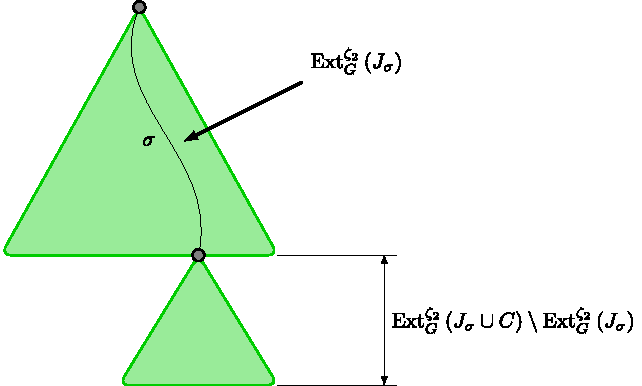
\includegraphics[width=\linewidth,height=0.78\textheight,keepaspectratio]{ccc2025-32-svg-01.pdf}\par



Figure 1: Modification of a branch.




\par\medskip\noindent\textbf{
5.3.3 Perfectness. Broken Branches}\par




We pick an assignment $\rho$ from distribution $\mathfrak{U}_{p,\zeta_{2}}$. By construction,
this assignment is $\zeta_{2}$-closed, and the witness of this property is $J_{\rho}\coloneqq J$,
where $J$ is a set from the algorithm that generates this assignment.\par




Note that by Chernoff bound:\par


\[\begin{gathered}
\Pr[|J|\geq 2pn]\leq\exp\left[-\frac{4}{3}pn\right]\leq\exp\left[-\frac{4}{3}%
\varepsilon r\right].
\end{gathered}\]


So we assume that $|J|<2pn$.\par




Consider some branch $\sigma\in B^{i}_{j}$ that is consistent with $\rho$. Note that:\par


\begin{itemize}


\item[] 
$\blacksquare$ 


$G^{\sigma}$ is a dependency graph of $A|_{\sigma}$;\par





\item[] 
$\blacksquare$ 


$G^{\sigma}$ is the $(r,\Delta,\zeta_{3})$-boundary expanders by Lemma
7.\par





\end{itemize}




Let us remind that $F_{\sigma}$ consists of locally consistent (wrt graph $G^{\sigma}$) terms of the
label of branch $\sigma\in B^{i}_{j}$.\par




We want to show that if $\mathrm{clv}_{G^{\sigma}}^{\zeta_{4}}\left(F_{\sigma}\right)>b_{i}$ then $\rho$ satisfies
$F_{\sigma}$ whp.\par




Since $\sigma\in B^{i}_{j}$ then $\mathrm{clv}_{G^{\sigma}}^{\zeta_{4}}\left(F\right)>b_{i}$. We apply Lemma
27 for graph $G^{\sigma}$, a collection of terms $F_{\sigma}$, and
$c\coloneqq\zeta_{3}$ and $\nu\coloneqq\zeta_{4}$ and get a sequence of terms
$T\coloneqq\{t_{1},\dots,t_{a}\}$ from $F$ such that:\par


\begin{itemize}


\item[] 
$\blacksquare$ 


for any $j\leq a$, $\mathrm{vars}(t_{j})$ is $\zeta_{4}$-closure independent of
$\bigcup\limits_{e=1}^{j-1}\mathrm{vars}(t_{e})$;\par





\item[] 
$\blacksquare$ 


$a\geq\frac{1}{(1+\frac{1}{\varepsilon})k}b_{i}>\frac{\varepsilon}{2k}b_{i}$.\par





\end{itemize}




The set $J$ contains the set $t_{j}$ with probability at least $p^{|t_{j}|}\geq p^{k}$. And since for
any $j,j^{\prime}\in[a]$: $t_{j}\cap t_{j^{\prime}}=\emptyset$ we can apply Chernoff bound and say:\par


\[\begin{gathered}
\displaystyle\Pr\left[J\text{ contains less than $\frac{1}{2}\cdot\frac{%
\varepsilon}{2k}b_{i}p^{k}$ terms of $T$ }\right] \displaystyle\leq\exp\left[-\frac{1}{8}\cdot\frac{1}{2}\cdot\frac{\varepsilon}%
{2k}b_{i}p^{k}\right] \\
\displaystyle\leq\exp\left[-\frac{1}{8}\cdot\frac{1}{2}\cdot\frac{\varepsilon}%
{2k}n^{\delta}\left(\frac{8}{p}\right)^{ik}p^{k}\right] \\
\displaystyle\leq\exp\left[-\frac{1}{8}\cdot\frac{1}{2}\cdot\frac{\varepsilon 8%
^{k}}{2k}n^{\delta}\left(\frac{8}{p}\right)^{(i-1)k}\right] \\
\displaystyle\leq\exp\left[-\frac{1}{8}\cdot\frac{1}{2}\cdot\frac{\varepsilon^%
{2}8^{k}}{2k}\log s_{i}\right] \\
\displaystyle\leq\left(\frac{1}{s_{i}}\right)^{4^{k}}.
\end{gathered}\]




Consider some $J$ that contains at least $\frac{\varepsilon}{4k}b_{i}p^{k}$ terms of $T$. Let $T^{\prime}\coloneqq\{t^{\prime}_{1},\dots,t^{\prime}_{a^{\prime}}\}$ be a subsequence of $T$ that consists of terms that are subsets of
$J$. Note that for any $j\leq a^{\prime}$, $\mathrm{vars}(t^{\prime}_{j})$ and $\bigcup\limits_{e=1}^{j-1}\mathrm{vars}(t^{\prime}_{e})$ are $\zeta_{4}$-closure-independent wrt $G^{\sigma}$. See fig. 2.\par
\par\noindent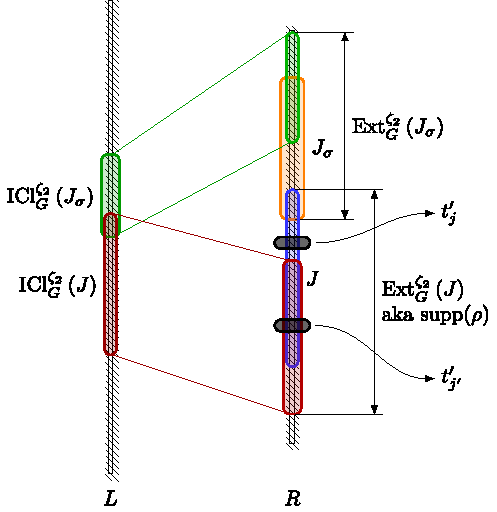
\includegraphics[width=\linewidth,height=0.78\textheight,keepaspectratio]{ccc2025-32-svg-02.pdf}\par



Figure 2: Graph $G$ and sets (proportions may be incorrect).



To estimate probability that we satisfy at least one term from $T^{\prime}$ we want to use Lemma 18. In order to do that, let us make the following observation.\par



% SOURCE-ID Thmtheorem20


\par\medskip\noindent\textbf{
$\blacktriangleright$ Remark 20.
}\par



\emph{A pair $(\mathrm{ICl}_{G}^{\zeta_{2}}\left(J\right),\operatorname*{supp}(\rho))$ is $\zeta_{5}$-reasonable wrt $G^{\sigma}$.}\par



% END-SOURCE-ID Thmtheorem20



\par\medskip\noindent\textbf{Proof.}\par




Note that $G^{\sigma}=(L\setminus\mathrm{ICl}_{G}^{\zeta_{2}}\left(J_{\sigma}\right),R%
\setminus\mathrm{Ext}_{G}^{\zeta_{2}}\left(J_{\sigma}\right),E)$. Hence if we erase the pair $(\mathrm{ICl}_{G}^{\zeta_{2}}\left(J\right),\operatorname*{supp}(\rho))$
from $G^{\sigma}$, the resulting graph will be $G^{\sigma,\rho}$ and the statement follows from Lemma
7.
$\blacktriangleleft$\par




Let $G^{\sigma}\coloneqq(L^{\sigma},R^{\sigma},E)$. For fixed $J$, assuming that $\rho$ is consistent
with $\sigma$, we may think that $\rho$ is taken from
$\mathfrak{U}_{\mathrm{Ext}_{G}^{\zeta_{2}}\left(J\right)\cap R^{\sigma}}$ and the Remark 20 states that it is a
locally consistent assignment wrt $G^{\sigma}$, which gives us an access to Lemma
18. So we apply Lemma 18 with the following parameters: a
graph $G^{\sigma}$, $J\coloneqq\operatorname*{supp}(\rho)\cap R^{\sigma}$ and a collection $T^{\prime}$. Here we use an
assumption that $|J|<2\varepsilon r$ and hence $|\operatorname*{supp}(\rho)|$ is at most $\left(1+\Delta\cdot\frac{1}{\varepsilon\Delta}\right)\cdot 2\varepsilon r\leq 2%
.1\cdot r\leq\varepsilon\Delta r$ by Lemma 6. We conclude that probability that $\rho$ does not satisfy any
term from $T^{\prime}$ is at most:\par


\[\begin{gathered}
\displaystyle\left(1-\frac{1}{2^{k}}\right)^{\frac{\varepsilon}{4k}b_{i+1}p^{k}} \displaystyle\leq\exp\left[-\frac{\varepsilon}{4k2^{k}}b_{i+1}p^{k}\right] \\
\displaystyle\leq\exp\left[-\frac{\varepsilon}{4k2^{k}}n^{\delta}\left(\frac{8%
}{p}\right)^{ik}p^{k}\right] \\
\displaystyle\leq\exp\left[-\frac{\varepsilon^{2}8^{k}}{8k2^{k}}\log s_{i}\right] \\
\displaystyle\leq\left(\frac{1}{s_{i}}\right)^{4^{k}}.
\end{gathered}\]





\par\medskip\noindent\textbf{Probability of Fail.}\par




We fail the process in two cases:\par


\begin{itemize}


\item[] 
$\blacksquare$ 


$J$ is too large and we cannot use our lemmas for expander graphs. That happens with
probability $\exp\left[-\frac{4}{3}\varepsilon r\right]$;\par





\item[] 
$\blacksquare$ 


$\rho$ does not map to $1$ any term in some branch $\sigma\in B^{i}_{j}$. That happens with
probability at most $\sum\limits_{i\in[k/\varepsilon]}|\bigcup\limits_{j=1}^{s}B^{i}_{j}|\cdot 2%
\left(\frac{1}{s_{i}}\right)^{4^{k}}$ (either $J$ does not cover enough terms or $\rho$
does not satisfy at least one of covered terms). To conclude the counting, note that $\left|\bigcup\limits_{j=1}^{s}B^{i}_{j}\right|\leq s_{i}$.\par





\end{itemize}


Hence whp our transformation satisfies perfectness for branches from all sets $B^{i}_{j}$.\par






\par\medskip\noindent\textbf{
5.3.4 Perfectness. Alive Branches}\par




This is the place where we use the properties of individual closure. Let us consider some $\sigma\in\mathrm{Br}^{*}_{T^{i}_{j}}\setminus B^{i}_{j}$ that is marked by a DNF $D$ and an arbitrary locally consistent term $t\in D$. Note that $\mathrm{clv}_{G^{\sigma}}^{\zeta_{2}}\left(D\right)\leq b_{i}$. Let $C$ be the set of variables on which the value
of $\mathrm{clv}_{G^{\sigma}}^{\zeta_{2}}\left(D\right)$ is achieved. At this iteration we split according to the variables in
some set $S\supseteq C$. Consider an assignment $\sigma^{\prime}$ to the variables
of $S$. Note that $|\mathrm{Ext}_{G^{\sigma}}^{\zeta_{4}}\left(t|_{\sigma^{\prime}}\right)|\leq|%
\mathrm{Ext}_{G^{\sigma}}^{\zeta_{4}}\left(t\right)|-1$ by the
definition of closure covering and Lemma 9. Again note that
$|\mathrm{Ext}_{G^{\sigma\cup\sigma^{\prime}}}^{\zeta_{4}}\left(t|_{\sigma^{%
\prime}}\right)|\leq|\mathrm{Ext}_{G^{\sigma}}^{\zeta_{4}}\left(t|_{\sigma^{%
\prime}}\right)|$ by
Lemma 9. Hence for any term $t^{\prime}$ that corresponds to some branch $\sigma^{\prime}\in\mathrm{Br}_{T^{i}_{j}}\setminus B^{i}_{j}$ and survives after $i+1$-th iteration we note that
$|\mathrm{Ext}_{G^{\sigma^{\prime}}}^{\zeta_{4}}\left(t^{\prime}\right)|$ is strictly less than $|\mathrm{Ext}_{G^{\sigma}}^{\zeta_{4}}\left(t\right)|$ where $t$ is
term in $\sigma\in\mathrm{Br}_{T^{i}_{j}}$ that generates $t^{\prime}$ after application of our transformation of the trees.\par




Note that for any term $t^{\prime\prime}$ that appears in the original proof
$|\mathrm{Ext}_{G}^{\zeta_{4}}\left(t^{\prime\prime}\right)|\leq\left(1+\frac{1%
}{3\varepsilon}\right)k\leq\frac{k}{\varepsilon}$ by
Lemma 6. Hence after $\frac{k}{\varepsilon}$ iterations for any locally consistent
term $t$: $|\mathrm{Ext}_{G^{\sigma}}^{\zeta_{4}}\left(t\right)|=0$, or in other words it is mapped to a constant and the
desired statement follows.\par





\par\medskip\noindent\textbf{
5.3.5 Lower Bound on Height}\par




Now we have a sequence of perfect trees $\{T^{k/\varepsilon+1}_{1},T^{k/\varepsilon+1}_{2},\dots,T^{k/\varepsilon+1}_{s}\}$ and we want to show non-existence of such sequence. We say that a
branch $\sigma\in\mathrm{Br}_{T^{k/\varepsilon+1}_{j}}$ has \textbf{survived} iff $\sigma$ is consistent with
$\rho$ and $\sigma\cup\rho$ is locally consistent.\par



% SOURCE-ID Thmtheorem21


\par\medskip\noindent\textbf{
$\blacktriangleright$ Remark 21.
}\par



\emph{In fact, one can extract a resolution proof of $A|_{\rho}$ of small enough width from these
trees, but it requires much more technical work and accuracy. And we believe that the direct proof
of the height lower bound is more useful for future generalizations.}\par



% END-SOURCE-ID Thmtheorem21



Let $T_{j}\coloneqq T^{k/\varepsilon+1}_{j}$. Note that $T_{j}$ strongly represents $D_{j}|_{\rho}$ by
construction. We consider a dag of the proof $\pi$. Starting from the vertex $s$ in this dag, we trace
the path $p$ to the initial clause. In the node $v\in p$ we maintain a partial assignment $\kappa_{v}$
such that:\par


\begin{itemize}


\item[] 
$\blacksquare$ 


$\kappa_{v}\in\mathrm{Br}^{*}_{T_{v}}\cup\mathrm{Br}^{0}_{T_{v}}$;\par





\item[] 
$\blacksquare$ 


$\kappa_{v}$ have survived.\par





\end{itemize}




Tree $T_{s}$ is a tree that consists of a single node marked by $0$ and we take $\kappa_{s}\coloneqq\emptyset$.\par




Consider a node $v$ of the dag of $\pi$. Assume that $D_{v}$ is derived from $D_{i_{1}},\dots,D_{i_{k}}$.
We have an assignment $\kappa_{v}$ that satisfies the required properties. Our goal is to find a branch
among branches of trees $T_{i_{1}},\dots,T_{i_{k}}$ that also satisfies the required properties. We will do
it by increasing $\kappa_{v}$ step by step. On each step we will have a closed assignment $\kappa\supseteq\kappa_{v}$ and a set $J_{\kappa}$ such that:\par




\begin{itemize}


\item[] 
$\blacksquare$ 


$\kappa$ and $\rho$ are consistent;\par





\item[] 
$\blacksquare$ 


$\operatorname*{supp}(\kappa)=\mathrm{Ext}_{G}^{\zeta_{2}}\left(J_{\kappa}\right)$;\par





\item[] 
$\blacksquare$ 


$\kappa$ satisfies $A^{\mathrm{ICl}_{G}^{\zeta_{2}}\left(J_{\kappa}\right)}$;\par





\item[] 
$\blacksquare$ 


$|\operatorname*{supp}(\kappa)|=o(r)$.\par





\end{itemize}




Note that assignment $\kappa_{v}\in\mathrm{Br}_{T_{v}}$ is closed. Hence the set $J_{\kappa_{v}}$ satisfies the required
properties, and in the beginning $\kappa$ is well-defined. Now we apply the following procedure to the
assignment $\kappa$.\par



\textbf{Algorithm 1}  Branch search.
\par\noindent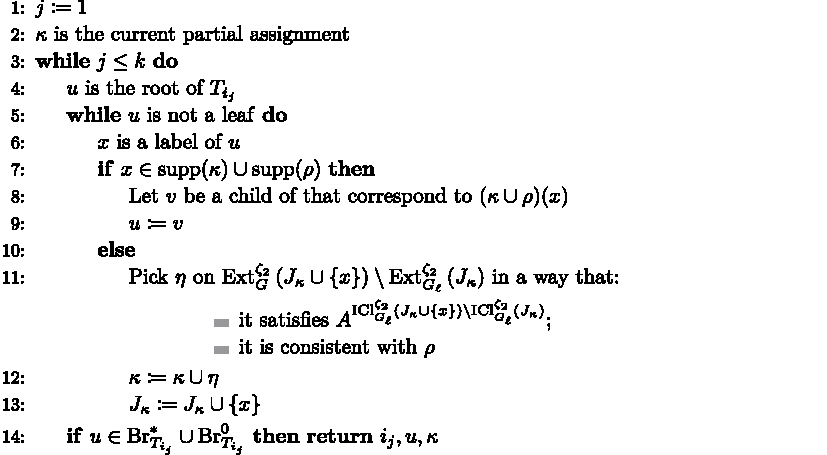
\includegraphics[width=\linewidth,height=0.78\textheight,keepaspectratio]{ccc2025-32-svg-03.pdf}\par



Note that height of the trees is at most $\frac{d_{k/\varepsilon+1}}{\varepsilon}=\frac{2}{\varepsilon}n^{\delta}\left(%
\frac{8}{p}\right)^{k^{2}/\varepsilon}=o(r/k)$ and hence
$\kappa$ has size $o(r)$ by construction and Lemma 6.\par




We have to show the existence of $\eta$ and that we stop on some iteration. We start with the existence.
Fix some iteration of the inner loop. Note that $\operatorname*{supp}(\kappa)=\mathrm{Ext}_{G}^{\zeta_{2}}\left(J_{\kappa}\right)$ and
$\operatorname*{supp}(\rho)=\mathrm{Ext}_{G}^{\zeta_{2}}\left(J_{\rho}\right)$ which by Lemma 7 implies that
$G^{\sigma,\rho}$ is an $(r,\Delta,\zeta_{5})$-expander. Moreover $G^{\sigma,\rho}$ is a dependency
graph of $A|_{\kappa\cup\rho}$. Hence by Lemma 11 there is a total assignment $\eta^{\prime}$
that satisfies $A^{\mathrm{ICl}_{G_{\ell}}^{\zeta_{2}}\left(J_{\kappa}\cup\{x\}\right)%
\setminus\mathrm{ICl}_{G_{\ell}}^{\zeta_{2}}\left(J_{\kappa}\right)}|_{\kappa%
\cup\rho}$. Let $\eta$ be a restriction of $\eta^{\prime}$ on
$\mathrm{Ext}_{G}^{\zeta_{2}}\left(J_{\kappa}\cup\{x\}\right)\setminus\mathrm{%
Ext}_{G_{\ell}}^{\zeta_{2}}\left(J_{\kappa}\right)$.\par




Now we want to show that we stop after some iteration. Note that:\par


\begin{itemize}


\item[] 
$\blacksquare$ 


$\kappa$ and $\rho$ are consistent (by construction);\par





\item[] 
$\blacksquare$ 


$\kappa$ is an extension of $\kappa_{v}$ (by construction);\par





\item[] 
$\blacksquare$ 


$\kappa\cup\rho$ satisfies $A^{\mathrm{ICl}_{G}^{\zeta_{2}}\left(J_{\kappa}\right)\cup\mathrm{ICl}_{G}^{%
\zeta_{2}}\left(J_{\rho}\right)}$
(by construction);\par





\item[] 
$\blacksquare$ 


For any $I$ of size at most $r$: $A^{I}|_{\rho\cup\kappa}$ is satisfiable (by Lemma
11).\par





\end{itemize}




For the sake of contradiction, assume that on each iteration of outer loop we found some leaf from
$\mathrm{Br}^{1}_{T_{i_{j}}}$. Consider three cases.\par


\begin{itemize}


\item[] 
$\blacksquare$ 


$D_{v}$ is obtained by using weakening or And-elimination rule from $D_{i_{1}}$. Assignment
$\kappa\cup\rho$ maps some term of $D_{i_{1}}$ to $1$ and hence it is also maps some term of
$D_{v}$ to $1$.\par





\item[] 
$\blacksquare$ 


$D_{v}$ is obtained by using And-introduction $\frac{F\vee\ell_{1},\dots,F\vee\ell_{w}}{F\vee(\bigwedge\limits_{i=0}^{w}\ell_%
{i})}$. If $\kappa\cup\rho$ maps some term $t\in F$ to
$1$, then $t\in D_{v}$ is also mapped to $1$. If $\kappa\cup\rho$ maps all $\ell_{j}$ to $1$
then $(\bigwedge\limits_{i=0}^{w}\ell_{i})\in D_{v}$ is also mapped to $1$.\par





\item[] 
$\blacksquare$ 


$D_{v}$ is obtained by using cut rule $\frac{F\vee(\bigwedge\limits_{i=0}^{w}\ell_{i}),G\vee(\bigvee\limits_{i=0}^{w}%
\neg\ell_{i})}{F\vee G}$. Note that $\kappa\cup\rho$ maps some
term $t\in F\vee(\bigwedge\limits_{i=0}^{w}\ell_{i})$ to $1$ and some term $t^{\prime}\in G\vee(\bigvee\limits_{i=0}^{w}\neg\ell_{i})$, hence $\kappa\cup\rho$ maps some term in $F\vee G=D_{v}$ to $1$.\par





\end{itemize}


In all cases we conclude that $\kappa\cup\rho$ maps some term $t\in D_{v}$ to $1$. But note that a pair
$(\mathrm{ICl}_{G}^{\zeta_{2}}\left(J_{\kappa}\right)\cup\mathrm{ICl}_{G}^{%
\zeta_{2}}\left(J_{\rho}\right),\mathrm{Ext}_{G}^{\zeta_{2}}\left(J_{\kappa}%
\right)\cup\mathrm{Ext}_{G}^{\zeta_{2}}\left(J_{\rho}\right))$ is $\zeta_{5}$-reasonable by Lemma 7, hence $\kappa\cup\rho$ is the witness of local satisfiability of $t$. That contradicts with the choice of branch
$\kappa_{v}$, since any term of $D_{v}$ is mapped by $\kappa_{v}$ either to constant $0$ or to locally
inconsistent term, and $\kappa\cup\rho$ is an extension of $\kappa_{v}$.\par




Our algorithm returns some triple $(i_{j},u,\kappa)$. We define $\kappa_{i_{j}}\coloneqq u$. Note that $\kappa_{i_{j}}\subseteq\kappa$ hence $\kappa_{i_{j}}\cup\rho$ does not violate any initial
clause and $\kappa_{i_{j}}\in\mathrm{Br}^{0}_{T_{i_{j}}}\cup\mathrm{Br}^{*}_{T_{i_{j}}}$.\par




By tracing the path in $\pi$ we reach a tree $T$ that strongly represents an initial clause $D$. We
have a branch $\kappa\in\mathrm{Br}_{T}$ such that:\par


\begin{itemize}


\item[] 
$\blacksquare$ 


$\kappa$ and $\rho$ are consistent;\par





\item[] 
$\blacksquare$ 


$\kappa\in\mathrm{Br}^{*}_{T}\cup\mathrm{Br}^{0}_{T}$, which implies that $\kappa$ violates $D$;\par





\item[] 
$\blacksquare$ 


$\kappa\cup\rho$ does not violate any initial clause.\par





\end{itemize}


That is a contradiction.\par







\par\medskip\noindent\textbf{
6 Application to Random Formulas}\par



% SOURCE-ID Thmtheorem22


\par\medskip\noindent\textbf{
\textbf{Theorem 22}\textbf{.}
}\par



\emph{Let $\Delta>120$, $\eta>0$ be arbitrary constants. If $\varphi\sim\varphi(m,n,\Delta)$
where $m\leq\eta n$, then there are constants $\delta,\nu>0$ such that whp any $\mathrm{Res}(k)$ proof of
$\varphi$ has size at least $2^{n^{\delta}}$ where $k\leq\nu\sqrt{\log{n}}$.}\par



% END-SOURCE-ID Thmtheorem22



\par\medskip\noindent\textbf{Proof.}\par




Applying Theorem 28, we conclude that the
dependency graph of our formula is an $(r,\Delta,0.95\Delta)$-boundary expander, where $r\coloneqq\delta n$ for some constant $\delta$ that depends only on $\eta$ and $\Delta$.\par




Note that:\par


\[\begin{gathered}
n^{\delta}\left(\frac{n}{8\varepsilon r}\right)^{k^{2}/\varepsilon}=n^{\delta}%
\left(\frac{1}{8\varepsilon\delta}\right)^{\nu^{2}\log n/\varepsilon}\leq n^{%
\delta}n^{\nu^{2}\log(1/8\varepsilon\delta)/\varepsilon}=o(r/k)
\end{gathered}\]


where the last inequality holds by the choice of $\nu$. The statement follows from Theorem 17.
$\blacktriangleleft$\par



% SOURCE-ID Thmtheorem23


\par\medskip\noindent\textbf{
\textbf{Theorem 23}\textbf{.}
}\par



\emph{For any $h>0$ there is $\Delta>0$ such that if $\varphi\sim\varphi(m,n,\Delta)$ where
$m\leq n\log^{h}n$, then there are constants $\delta,\nu>0$ such that whp any $\mathrm{Res}(k)$ proof of
$\varphi$ has size at least $2^{n^{\delta}}$ where $k\leq\nu\sqrt{\frac{\log{n}}{\log\log n}}$.}\par



% END-SOURCE-ID Thmtheorem23




\par\medskip\noindent\textbf{Proof.}\par




Applying Theorem 29 we conclude that there is $\Delta>0$ such that
dependency graph of our formula is an $(r,\Delta,0.95\Delta)$-boundary expander where $r\coloneqq n/\log^{\ell}n$ for some constant $\ell$ that depends only on $h$ and $\Delta$.\par




Note that:\par


\[\begin{gathered}
n^{\delta}\left(\frac{n}{8\varepsilon r}\right)^{k^{2}/\varepsilon}=n^{\delta}%
\left(\frac{\log^{\ell}n}{8\varepsilon}\right)^{\nu^{2}\log n/\varepsilon\log%
\log n}\leq n^{\delta}n^{\nu^{2}\ell\log(1/8\varepsilon)/\varepsilon}=o(r/k)
\end{gathered}\]


where the last inequality holds by the choice of $\nu$. The statement follows from Theorem 17.
$\blacktriangleleft$\par



% SOURCE-ID Thmtheorem24


\par\medskip\noindent\textbf{
\textbf{Theorem 24}\textbf{.}
}\par



\emph{For any $h>0$ there is $\Delta>0$ such that if $\varphi\sim\varphi(m,n,\Delta)$ where
$m\leq n^{h}$, then for any constant $k$ there is constant $\delta>0$ such that whp any $\mathrm{Res}(k)$
proof of $\varphi$ has size at least $2^{n^{\delta}}$.}\par



% END-SOURCE-ID Thmtheorem24




\par\medskip\noindent\textbf{Proof.}\par




Applying Theorem 30 we can choose any constant $\delta^{\prime}>0$ and $\Delta>0$
that depends only on $\delta$ such that dependency graph of our formula is an $(r,\Delta,0.95\Delta)$-boundary expander where $r\coloneqq n^{1-\delta^{\prime}}$.\par




Note that:\par


\[\begin{gathered}
n^{\delta}\left(\frac{n}{8\varepsilon r}\right)^{k^{2}/\varepsilon}=n^{\delta}%
\left(\frac{n^{\delta^{\prime}}}{8\varepsilon}\right)^{k^{2}/\varepsilon}\leq n%
^{\delta}n^{\delta^{\prime}k^{2}\log(1/8\varepsilon)/\varepsilon}=o(r/k)
\end{gathered}\]


where the last inequality holds by the choice of $\delta^{\prime}$. The statement follows from Theorem 17.
$\blacktriangleleft$\par



% SOURCE-ID Thmtheorem25


\par\medskip\noindent\textbf{
\textbf{Theorem 25}\textbf{.}
}\par



\emph{For any $h>0$ there are $\delta,\nu>0$ such that if $\varphi\sim\varphi(m,n,\Delta)$ where
$m\leq n^{\log\log^{h}n}$ and $\Delta\coloneqq\log n$, then whp any $\mathrm{Res}(k)$ proof of $\varphi$ has
size at least $2^{n^{\delta}}$ where $k\leq\nu\sqrt{\frac{\log{n}}{\log\log n}}$.}\par



% END-SOURCE-ID Thmtheorem25




\par\medskip\noindent\textbf{Proof.}\par




Applying Theorem 31 we conclude that dependency graph of our formula is an
$(r,\Delta,0.95\Delta)$-boundary expander where $r\coloneqq n/\log^{\ell}n$ for some constant
$\ell$ that depends only on $h$.\par




Note that:\par


\[\begin{gathered}
n^{\delta}\left(\frac{n}{8\varepsilon r}\right)^{k^{2}/\varepsilon}=n^{\delta}%
\left(\frac{\log^{\ell}n}{8\varepsilon}\right)^{\nu^{2}\log n/\varepsilon\log%
\log n}\leq n^{\delta}n^{\nu^{2}\ell\log(1/8\varepsilon)/\varepsilon}=o(r/k)
\end{gathered}\]


where the last inequality holds by the choice of $\nu$. The statement follows from Theorem 17.
$\blacktriangleleft$\par






\par\medskip\noindent\textbf{References}\par



\begin{itemize}


\item[] 
[1]

Jackson Abascal, Venkatesan Guruswami, and Pravesh K. Kothari.


Strongly refuting all semi-random boolean csps.


In Dániel Marx, editor, \emph{Proceedings of the 2021 ACM-SIAM
Symposium on Discrete Algorithms, SODA 2021, Virtual Conference, January 10
- 13, 2021}, pages 454–472. SIAM, 2021.


doi:10.1137/1.9781611976465.28.





\item[] 
[2]

Miklós Ajtai.


The complexity of the pigeonhole principle.


\emph{Combinatorica}, 14(4):417–433, 1994.


doi:10.1007/BF01302964.





\item[] 
[3]

Michael Alekhnovich.


Lower bounds for k-dnf resolution on random 3-cnfs.


\emph{Comput. Complex.}, 20(4):597–614, 2011.


doi:10.1007/s00037-011-0026-0.





\item[] 
[4]

Michael Alekhnovich, Eli Ben-Sasson, Alexander A. Razborov, and Avi Wigderson.


Pseudorandom generators in propositional proof complexity.


\emph{SIAM J. Comput.}, 34(1):67–88, 2004.


doi:10.1137/S0097539701389944.





\item[] 
[5]

Michael Alekhnovich and Alexander A. Razborov.


Lower bounds for polynomial calculus: Non-binomial case.


\emph{Proceedings of the Steklov Institute of Mathematics},
242:18–35, 2003.


Available at
http://people.cs.uchicago.edu/˜razborov/files/misha.pdf. Preliminary
version in \emph{FOCS ’01}.





\item[] 
[6]

Sarah R. Allen, Ryan O’Donnell, and David Witmer.


How to refute a random CSP.


In Venkatesan Guruswami, editor, \emph{IEEE 56th Annual Symposium on
Foundations of Computer Science, FOCS 2015, Berkeley, CA, USA, 17-20
October, 2015}, pages 689–708. IEEE Computer Society, 2015.


doi:10.1109/FOCS.2015.48.





\item[] 
[7]

Omar Alrabiah, Venkatesan Guruswami, Pravesh K. Kothari, and Peter Manohar.


A near-cubic lower bound for 3-query locally decodable codes from
semirandom CSP refutation.


In Barna Saha and Rocco A. Servedio, editors, \emph{Proceedings of the
55th Annual ACM Symposium on Theory of Computing, STOC 2023, Orlando, FL,
USA, June 20-23, 2023}, pages 1438–1448. ACM, 2023.


doi:10.1145/3564246.3585143.





\item[] 
[8]

Albert Atserias, Ilario Bonacina, Susanna F. de Rezende, Massimo Lauria, Jakob
Nordström, and Alexander A. Razborov.


Clique is hard on average for regular resolution.


In Ilias Diakonikolas, David Kempe, and Monika Henzinger, editors,
\emph{Proceedings of the 50th Annual ACM SIGACT Symposium on Theory of
Computing, STOC 2018, Los Angeles, CA, USA, June 25-29, 2018}, pages
866–877. ACM, 2018.


doi:10.1145/3188745.3188856.





\item[] 
[9]

Albert Atserias, Maria Luisa Bonet, and Juan Luis Esteban.


Lower bounds for the weak pigeonhole principle and random formulas
beyond resolution.


\emph{Inf. Comput.}, 176(2):136–152, 2002.


doi:10.1006/inco.2002.3114.





\item[] 
[10]

Paul Beame, Russell Impagliazzo, Jan Krajícek, Toniann Pitassi, and
Pavel Pudlák.


Lower bound on hilbert’s nullstellensatz and propositional proofs.


In \emph{35th Annual Symposium on Foundations of Computer Science,
Santa Fe, New Mexico, USA, 20-22 November 1994}, pages 794–806, 1994.


doi:10.1109/SFCS.1994.365714.





\item[] 
[11]

Paul Beame, Richard M. Karp, Toniann Pitassi, and Michael E. Saks.


The efficiency of resolution and davis–putnam procedures.


\emph{SIAM J. Comput.}, 31(4):1048–1075, 2002.


doi:10.1137/S0097539700369156.





\item[] 
[12]

Eli Ben-Sasson.


\emph{Expansion in proof complexity}.


PhD thesis, Hebrew University of Jerusalem, Israel, 2001.


URL:
https://huji-primo.hosted.exlibrisgroup.com/permalink/f/13ns5ae/972HUJI\_ALMA21159933340003701.





\item[] 
[13]

Eli Ben-Sasson and Russell Impagliazzo.


Random cnf’s are hard for the polynomial calculus.


In \emph{40th Annual Symposium on Foundations of Computer Science,
FOCS ’99, 17-18 October, 1999, New York, NY, USA}, pages 415–421. IEEE
Computer Society, 1999.


doi:10.1109/SFFCS.1999.814613.





\item[] 
[14]

Eli Ben-Sasson and Avi Wigderson.


Short proofs are narrow – resolution made simple.


\emph{J. ACM}, 48(2):149–169, 2001.


doi:10.1145/375827.375835.





\item[] 
[15]

Vašek Chvátal and Endre Szemerédi.


Many hard examples for resolution.


\emph{J. ACM}, 35(4):759–768, October 1988.


doi:10.1145/48014.48016.





\item[] 
[16]

Susanna F. de Rezende, Jakob Nordström, Kilian Risse, and Dmitry Sokolov.


Exponential resolution lower bounds for weak pigeonhole principle and
perfect matching formulas over sparse graphs.


\emph{CoRR}, abs/1912.00534, 2019.


arXiv:1912.00534.





\item[] 
[17]

Susanna F. de Rezende, Aaron Potechin, and Kilian Risse.


Clique is hard on average for unary sherali-adams.


In \emph{64th IEEE Annual Symposium on Foundations of Computer
Science, FOCS 2023, Santa Cruz, CA, USA, November 6-9, 2023}, pages 12–25.
IEEE, 2023.


doi:10.1109/FOCS57990.2023.00008.





\item[] 
[18]

Uriel Feige.


Relations between average case complexity and approximation
complexity.


In \emph{Proceedings of the 17th Annual IEEE Conference on
Computational Complexity, Montréal, Québec, Canada, May 21-24,
2002}, page 5. IEEE Computer Society, 2002.


doi:10.1109/CCC.2002.10006.





\item[] 
[19]

Uriel Feige, Jeong Han Kim, and Eran Ofek.


Witnesses for non-satisfiability of dense random 3cnf formulas.


In \emph{47th Annual IEEE Symposium on Foundations of Computer
Science (FOCS 2006), 21-24 October 2006, Berkeley, California, USA,
Proceedings}, pages 497–508. IEEE Computer Society,
2006.


doi:10.1109/FOCS.2006.78.





\item[] 
[20]

Noah Fleming, Denis Pankratov, Toniann Pitassi, and Robert Robere.


Random $\Theta$(log n)-cnfs are hard for cutting planes.


In Chris Umans, editor, \emph{58th IEEE Annual Symposium on
Foundations of Computer Science, FOCS 2017, Berkeley, CA, USA, October
15-17, 2017}, pages 109–120. IEEE Computer Society, 2017.


doi:10.1109/FOCS.2017.19.





\item[] 
[21]

Konstantinos Georgiou, Avner Magen, and Madhur Tulsiani.


Optimal sherali-adams gaps from pairwise independence.


In Irit Dinur, Klaus Jansen, Joseph Naor, and José Rolim,
editors, \emph{Approximation, Randomization, and Combinatorial Optimization.
Algorithms and Techniques}, pages 125–139, Berlin, Heidelberg, 2009.
Springer Berlin Heidelberg.


doi:10.1007/978-3-642-03685-9\_10.





\item[] 
[22]

Dima Grigoriev.


Linear lower bound on degrees of positivstellensatz calculus proofs
for the parity.


\emph{Theoretical Computer Science}, 259(1):613–622, 2001.


doi:10.1016/S0304-3975(00)00157-2.





\item[] 
[23]

Venkatesan Guruswami, Pravesh K. Kothari, and Peter Manohar.


Algorithms and certificates for boolean CSP refutation: smoothed is
no harder than random.


In Stefano Leonardi and Anupam Gupta, editors, \emph{STOC ’22: 54th
Annual ACM SIGACT Symposium on Theory of Computing, Rome, Italy, June 20
- 24, 2022}, pages 678–689. ACM, 2022.


doi:10.1145/3519935.3519955.





\item[] 
[24]

Johan Håstad.


On small-depth frege proofs for tseitin for grids.


\emph{J. ACM}, 68(1):1:1–1:31, 2021.


doi:10.1145/3425606.





\item[] 
[25]

Pavel Hrubes and Pavel Pudlák.


Random formulas, monotone circuits, and interpolation.


In Chris Umans, editor, \emph{58th IEEE Annual Symposium on
Foundations of Computer Science, FOCS 2017, Berkeley, CA, USA, October
15-17, 2017}, pages 121–131. IEEE Computer Society, 2017.


doi:10.1109/FOCS.2017.20.





\item[] 
[26]

Pravesh K. Kothari and Peter Manohar.


An exponential lower bound for linear 3-query locally correctable
codes.


In Bojan Mohar, Igor Shinkar, and Ryan O’Donnell, editors, \emph{Proceedings of the 56th Annual ACM Symposium on Theory of Computing, STOC
2024, Vancouver, BC, Canada, June 24-28, 2024}, pages 776–787. ACM, 2024.


doi:10.1145/3618260.3649640.





\item[] 
[27]

Pravesh K. Kothari, Ryuhei Mori, Ryan O’Donnell, and David Witmer.


Sum of squares lower bounds for refuting any CSP.


In Hamed Hatami, Pierre McKenzie, and Valerie King, editors, \emph{Proceedings of the 49th Annual ACM SIGACT Symposium on Theory of
Computing, STOC 2017, Montreal, QC, Canada, June 19-23, 2017}, pages
132–145. ACM, 2017.


doi:10.1145/3055399.3055485.





\item[] 
[28]

Jan Krajíček.


On the weak pigeonhole principle.


\emph{Fundamenta Mathematicae}, 170:123–140, January 2001.


doi:10.4064/fm170-1-8.





\item[] 
[29]

Sebastian Müller and Iddo Tzameret.


Short propositional refutations for dense random 3cnf formulas.


\emph{Ann. Pure Appl. Log.}, 165(12):1864–1918, 2014.


doi:10.1016/j.apal.2014.08.001.





\item[] 
[30]

Ryan O’Donnell.


\emph{Analysis of Boolean Functions}.


Cambridge University Press, 2014.


doi:10.1017/CBO9781139814782.





\item[] 
[31]

Shuo Pang.


Large clique is hard on average for resolution.


In Rahul Santhanam and Daniil Musatov, editors, \emph{Computer Science
- Theory and Applications - 16th International Computer Science Symposium in
Russia, CSR 2021, Sochi, Russia, June 28 - July 2, 2021, Proceedings},
volume 12730 of \emph{Lecture Notes in Computer Science}, pages 361–380.
Springer, 2021.


doi:10.1007/978-3-030-79416-3\_22.





\item[] 
[32]

Prasad Raghavendra, Satish Rao, and Tselil Schramm.


Strongly refuting random csps below the spectral threshold.


In Hamed Hatami, Pierre McKenzie, and Valerie King, editors, \emph{Proceedings of the 49th Annual ACM SIGACT Symposium on Theory of
Computing, STOC 2017, Montreal, QC, Canada, June 19-23, 2017}, pages
121–131. ACM, 2017.


doi:10.1145/3055399.3055417.





\item[] 
[33]

Alexander A. Razborov.


Pseudorandom generators hard for k-dnf resolution and polynomial
calculus resolution.


\emph{Ann. of Math.}, 181:415–472, 2015.


doi:10.4007/annals.2015.181.2.1.





\item[] 
[34]

Grant Schoenebeck.


Linear level lasserre lower bounds for certain k-csps.


In \emph{49th Annual IEEE Symposium on Foundations of Computer
Science, FOCS 2008, October 25-28, 2008, Philadelphia, PA, USA}, pages
593–602. IEEE Computer Society, 2008.


doi:10.1109/FOCS.2008.74.





\item[] 
[35]

Nathan Segerlind, Samuel R. Buss, and Russell Impagliazzo.


A switching lemma for small restrictions and lower bounds for k-dnf
resolution.


\emph{SIAM J. Comput.}, 33(5):1171–1200, 2004.


doi:10.1137/S0097539703428555.





\item[] 
[36]

Dmitry Sokolov.


(semi)algebraic proofs over $\pm$1 variables.


In Konstantin Makarychev, Yury Makarychev, Madhur Tulsiani, Gautam
Kamath, and Julia Chuzhoy, editors, \emph{Proccedings of the 52nd Annual ACM
SIGACT Symposium on Theory of Computing, STOC 2020, Chicago, IL, USA,
June 22-26, 2020}, pages 78–90. ACM, 2020.


doi:10.1145/3357713.3384288.





\item[] 
[37]

Dmitry Sokolov.


Random (log n)-cnf are hard for cutting planes (again).


In Bojan Mohar, Igor Shinkar, and Ryan O’Donnell, editors, \emph{Proceedings of the 56th Annual ACM Symposium on Theory of Computing, STOC
2024, Vancouver, BC, Canada, June 24-28, 2024}, pages 2008–2015. ACM,
2024.


doi:10.1145/3618260.3649636.





\item[] 
[38]

Salil P. Vadhan.


\emph{Pseudorandomness}.


Now Publishers Inc., Hanover, MA, USA, 2012.





\end{itemize}




\par\medskip\noindent\textbf{
Appendix A Chernoff Bound}\par



% SOURCE-ID Thmtheorem26


\par\medskip\noindent\textbf{
\textbf{Lemma 26}\textbf{ }(Chernoff bound)\textbf{.}
}\par



\emph{Let $X_{1},\dots,X_{n}$ be independent random variables taking values in $\{0,1\}$, $X\coloneqq\sum X_{i}$ and $\mu\coloneqq\mathbb{E}[X]$.}\par


\begin{itemize}


\item[] 
$\blacksquare$ 


$\Pr[X\leq(1-\delta)\mu]\leq\exp\left[-\frac{\delta^{2}}{2}\mu\right]$\emph{;}\par





\item[] 
$\blacksquare$ 


$\Pr[X\geq(1+\delta)\mu]\leq\exp\left[-\frac{\delta^{2}}{2+\delta}\mu\right]$\emph{.}\par





\end{itemize}



% END-SOURCE-ID Thmtheorem26




\par\medskip\noindent\textbf{
Appendix B Graph Properties}\par



% SOURCE-ID Thmtheorem27


\par\medskip\noindent\textbf{
\textbf{Lemma 27}\textbf{.}
}\par



\emph{Let $G\coloneqq(L,R,E)$ be an $(r,\Delta,c)$-boundary expander, $\mathcal{S}\coloneqq\{S_{1},S_{2},\dots,S_{\ell}\}$ be a collection of subsets of $R$ such that $|S_{i}|\leq k$. Then for each $\nu<c$ it is possible to pick a sequence $\{B_{1},\dots,B_{h}\}$ where:}\par


\begin{itemize}


\item[] 
$\blacksquare$ 


\emph{for all }$i\in[h]$\emph{ there is }$j\in[\ell]$\emph{ such that }$B_{i}=S_{j}$\emph{;}\par





\item[] 
$\blacksquare$ 


$B_{i}$\emph{ is }$\nu$\emph{-closure-independent of }$\bigcup\limits_{j=1}^{i-1}B_{j}$\emph{;}\par





\item[] 
$\blacksquare$ 


$h\geq\min\left(r/k,\frac{\mathrm{clv}\left(\mathcal{S}\right)}{\left(1+\frac{%
\Delta}{c-\nu}\right)k}\right)$\emph{.}\par





\end{itemize}



% END-SOURCE-ID Thmtheorem27



\par\medskip\noindent\textbf{Proof.}\par




Let us start picking $B$’s in a greedy way. Suppose we picked $i$
terms for some $0<i<r/k$, and we are not able to pick the
term $i+1$. This means that the set of vertices
$\mathrm{Ext}^{\nu}\left(\bigcup\limits_{j<i}B_{j}\right)$ is a closure covering
for $\mathcal{S}$.\par


\[\begin{gathered}
\displaystyle\mathrm{clv}\left(\mathcal{S}\right) \displaystyle\leq|\mathrm{Ext}^{\nu}\left(\bigcup\limits_{j<i}B_{j}\right)| \\
\displaystyle\leq\left(1+\frac{\Delta}{c-\nu}\right)|\bigcup\limits_{j<i}B_{j}| \\
\displaystyle\leq\left(1+\frac{\Delta}{c-\nu}\right)ik,
\end{gathered}\]


hence $i\geq\frac{\mathrm{clv}\left(\mathcal{S}\right)}{\left(1+\frac{\Delta}{c-\nu}%
\right)k}$.
$\blacktriangleleft$\par






\par\medskip\noindent\textbf{
Appendix C Random Graph is an Expander}\par




For $m,n,\Delta\in\mathbb{N}$, we denote by $\mathfrak{G}(m,n,\Delta)$ the distribution over
bipartite graphs with disjoint vertex sets $U\coloneqq\{u_{1},\dots,u_{m}\}$ and $V\coloneqq\{v_{1},\dots,v_{n}\}$ where the neighbourhood of a vertex $u\in U$ is chosen by sampling a subset of size
$\Delta$ uniformly at random from $V$.\par




Let $G$ be a randomly sampled graph from $\mathfrak{G}(m,n,\Delta)$ and $\varepsilon<1/2$. We
estimate the probability that $G$ is not an $(r,\Delta,(1-\varepsilon)\Delta)$-boundary expander
for some parameter $r$.\par




Let $G\coloneqq(U,V,E)$. We first estimate the probability that a set $S\subseteq U$ of size at most
$r$ violates the boundary expansion. For brevity, let us write $s=|S|$ and $c=(1-\frac{\varepsilon}{2})\Delta$. The probability that $S$ violates the boundary expansion can be bounded
by:\par


\[\begin{gathered}
\displaystyle\Pr[|\partial(S)|<(1-\varepsilon)\Delta s] \displaystyle\leq\Pr[|\mathrm{N}\left(S\right)<cs] \\
\displaystyle\leq\binom{n}{cs}\cdot\left(\frac{\binom{cs}{\Delta}}{\binom{n}{%
\Delta}}\right)^{s} \\
\displaystyle\leq\binom{n}{cs}\cdot\left(\frac{cs}{n}\right)^{\Delta s} \\
\displaystyle\leq\left[\left(\frac{en}{cs}\right)^{c}\cdot\left(\frac{cs}{n}%
\right)^{\Delta}\right]^{s}
\end{gathered}\]


Hence, the probability that $G$ is not a boundary expander can be bounded by\par


\[\begin{gathered}
\displaystyle\Pr[G\text{ is not an expander}] \displaystyle\leq\sum\limits_{s\in[r]}\binom{m}{s}\left[\left(\frac{en}{cs}%
\right)^{c}\cdot\left(\frac{cs}{n}\right)^{\Delta}\right]^{s} \\
\displaystyle\leq\sum\limits_{s\in[r]}\left(\frac{me}{s}\right)^{s}\left[\left%
(\frac{en}{cs}\right)^{c}\cdot\left(\frac{cs}{n}\right)^{\Delta}\right]^{s} \\
\displaystyle\leq\sum\limits_{s\in[r]}\left[\frac{me}{s}\left(\frac{en}{cs}%
\right)^{c}\cdot\left(\frac{cs}{n}\right)^{\Delta}\right]^{s} \\
\displaystyle\leq\sum\limits_{s\in[r]}\left[e^{1+c}\frac{m}{s}\left(\frac{cs}{%
n}\right)^{\frac{\varepsilon}{2}\Delta}\right]^{s}
\end{gathered}\]




Now we can formulate some classical results about the existence of expander graphs.\par



% SOURCE-ID Thmtheorem28


\par\medskip\noindent\textbf{
\textbf{Theorem 28}\textbf{.}
}\par



\emph{Let $\frac{1}{2}>\varepsilon>0$, $\Delta>6/\varepsilon$ be arbitrary constants. If $m\leq\eta n$, there is a constant $\delta>0$ such that whp for $r\coloneqq\delta n$ a randomly sampled
graph $G\sim\mathfrak{G}(m,n,\Delta)$ is an $(r,\Delta,(1-\varepsilon)\Delta)$-boundary
expander.}\par



% END-SOURCE-ID Thmtheorem28



\par\medskip\noindent\textbf{Proof.}\par




Let $c\coloneqq(1-\frac{\varepsilon}{2})\Delta$ and $\delta^{\prime}\coloneqq\frac{\Delta r}{n}$. Note
that $G$ is not a boundary expander with probability at most:\par


\[\begin{gathered}
\displaystyle\sum\limits_{s\in[r]}\left[e^{1+c}\frac{m}{s}\left(\frac{cs}{n}%
\right)^{\frac{\varepsilon}{2}\Delta}\right]^{s} \displaystyle\leq\sum\limits_{s\in[r]}\left[e^{1+c}\frac{\eta n}{s}\left(\frac%
{cs}{n}\right)^{\frac{\varepsilon}{2}\Delta}\right]^{s} \\
\displaystyle=\sum\limits_{s\in[r]}\left[e^{1+c}\eta c\left(\frac{cs}{n}\right%
)^{\frac{\varepsilon}{2}\Delta-1}\right]^{s} \\
\displaystyle\leq\sum\limits_{s\in[r]}\left[e^{1+c}\eta c\left(\delta^{\prime}%
\right)^{\frac{\varepsilon}{2}\Delta-1}\right]^{s}.
\end{gathered}\]




And if $\Delta>6/\varepsilon$ we can choose $\delta$ to make sure that this sum is at most
$0.01$.
$\blacktriangleleft$\par



% SOURCE-ID Thmtheorem29


\par\medskip\noindent\textbf{
\textbf{Theorem 29}\textbf{.}
}\par



\emph{Let $m\leq n\log^{h}n$ for some universal constant $h$ and $\varepsilon\coloneqq 0.01$. For any
constant $\ell>0$ there is a constant $\Delta>0$ such that whp for $r\coloneqq n/\log^{\ell}n$ a randomly sampled graph $G\sim\mathfrak{G}(m,n,\Delta)$ is an $(r,\Delta,(1-\varepsilon)\Delta)$-boundary expander.}\par



% END-SOURCE-ID Thmtheorem29




\par\medskip\noindent\textbf{Proof.}\par




Let $c\coloneqq(1-\frac{\varepsilon}{2})\Delta$. Note that $G$ is not a boundary expander with
probability at most:\par


\[\begin{gathered}
\displaystyle\sum\limits_{s\in[r]}\left[e^{1+c}\frac{m}{s}\left(\frac{cs}{n}%
\right)^{\frac{\varepsilon}{2}\Delta}\right]^{s} \displaystyle=\sum\limits_{s\in[r]}\left[e^{1+c}\frac{mc}{n}\left(\frac{cs}{n}%
\right)^{\frac{\varepsilon}{2}\Delta-1}\right]^{s}. \\
\displaystyle\leq\sum\limits_{s\in[r]}\left[e^{1+c}c\log^{h}n\left(\Delta\log^%
{-\ell}n\right)^{\frac{\varepsilon}{2}\Delta-1}\right]^{s}.
\end{gathered}\]


And if $\Delta>\frac{6(h+\ell)}{\varepsilon\ell}$ this sum is $o(1)$.
$\blacktriangleleft$\par



% SOURCE-ID Thmtheorem30


\par\medskip\noindent\textbf{
\textbf{Theorem 30}\textbf{.}
}\par



\emph{Let $m\leq n^{h}$ for some universal constant $h$ and $\varepsilon\coloneqq 0.01$. For any constant
$\delta>0$ there is a constant $\Delta>0$ such that whp for $r\coloneqq n^{1-\delta}$ a
randomly sampled graph $G\sim\mathfrak{G}(m,n,\Delta)$ is an $(r,\Delta,(1-\varepsilon)\Delta)$-boundary expander.}\par



% END-SOURCE-ID Thmtheorem30




\par\medskip\noindent\textbf{Proof.}\par




Let $c=(1-\frac{\varepsilon}{2})\Delta$. Note that $G$ is not a boundary expander with
probability at most:\par


\[\begin{gathered}
\displaystyle\sum\limits_{s\in[r]}\left[e^{1+c}\frac{m}{s}\left(\frac{cs}{n}%
\right)^{\frac{\varepsilon}{2}\Delta}\right]^{s}\leq \displaystyle\sum\limits_{s\in[r]}\left[e^{1+c}n^{h}\left(n^{-\delta/2}\right)%
^{\frac{\varepsilon}{2}\Delta}\right]^{s}.
\end{gathered}\]


And if $\Delta>\frac{6h}{\varepsilon\delta}$ this sum is $o(1)$.
$\blacktriangleleft$\par



% SOURCE-ID Thmtheorem31


\par\medskip\noindent\textbf{
\textbf{Theorem 31}\textbf{.}
}\par



\emph{Let $m\leq n^{\log\log^{h}n}$ for some universal constant $h$, $\varepsilon\coloneqq 0.01$. For
any constant $\delta>0$ there is a constant $\ell>0$ such that whp for $r\coloneqq n/\log^{\ell}n$ a randomly sampled graph $G\sim\mathfrak{G}(m,n,\Delta)$ is an $(r,\Delta,(1-\varepsilon)\Delta)$-boundary expander where $\Delta\coloneqq\log n$.}\par



% END-SOURCE-ID Thmtheorem31




\par\medskip\noindent\textbf{Proof.}\par




Let $c=(1-\frac{\varepsilon}{2})\Delta$. Note that $G$ is not a boundary expander with
probability at most:\par


\[\begin{gathered}
\displaystyle\sum\limits_{s\in[r]}\left[e^{1+c}\frac{m}{s}\left(\frac{cs}{n}%
\right)^{\frac{\varepsilon}{2}\Delta}\right]^{s}\leq \displaystyle\sum\limits_{s\in[r]}\left[e^{1+c}n^{\log\log^{h}n}\left(\log^{-%
\ell/2}n\right)^{\frac{\varepsilon}{2}\Delta}\right]^{s}.
\end{gathered}\]


And if $\ell>\frac{6h}{\varepsilon}$ this sum is $o(1)$.
$\blacktriangleleft$\par






\par\medskip\noindent\textbf{
Appendix D Proof of Lemma 11
}\par



% SOURCE-ID Thmtheorem32


\par\medskip\noindent\textbf{
\textbf{Lemma 32}\textbf{.}
}\par



\emph{Let $A$ be a linear system based on a graph $G\coloneqq(L,R,E)$ that is an $(r,\Delta,c)$-expander. If $\sigma$ is a locally consistent assignment, then for any $I$ of size at most $r$
the system $A^{I}|_{\sigma}$ is satisfiable.}\par



% END-SOURCE-ID Thmtheorem32



\par\medskip\noindent\textbf{Proof.}\par




Let a pair $(S,T)$ be a witness of the consistency of $\sigma$. So $(S,T)$ is a $\zeta$-reasonable
pair for some $\zeta>0$. Let $\sigma^{\prime}$ be an extension of $\sigma$ on $T\cup\mathrm{N}\left(S\right)$ such that
$A^{S}|_{\sigma^{\prime}}$ is satisfied (it exists since $A^{S}|_{\sigma}$ is satisfiable).\par




Pick an arbitrary set $I$ of size at most $r$. Note that $\sigma^{\prime}$ satisfies all constraints from $I\cap S$. Let $I^{\prime}\coloneqq I\setminus S$. Consider a graph $G^{\prime}$ obtained by removing a pair $(S,T\cup\mathrm{N}\left(S\right))$, that is $(r,\Delta,\zeta)$-boundary expander. By Lemma 4
(applied to $G^{\prime}$) there is an enumeration $I^{\prime}=\{v_{1},v_{2},\dots,v_{|I^{\prime}|}\}$ and a
partition $\bigsqcup\limits_{i}R_{i}=\mathrm{N}_{G^{\prime}}\left(I^{\prime}\right)$ such that:\par


\begin{itemize}


\item[] 
$\blacksquare$ 


$R_{i}=\mathrm{N}\left(v_{i}\right)\setminus\left(\bigcup\limits_{j=1}^{i-1}%
\mathrm{N}\left(v_{j}\right)\right)$;\par





\item[] 
$\blacksquare$ 


$|\partial(v_{i})\cap R_{i}|\geq\zeta$.\par





\end{itemize}


For each $i\in[|I^{\prime}|]$ we extend $\sigma^{\prime}$ on $R_{i}$ by choosing an arbitrary assignment that satisfies
constraint $A^{v_{i}}|_{\sigma^{\prime}}$. Since $|\partial(v_{i})\cap R_{i}|>0$ there is at least one such assignment and we are
done.
$\blacktriangleleft$\par




\par




\end{document}
